\section{Generating Code for Patterns}

\subsection{Introduction}

\begin{enumerate}
\item
`isa` procedure that accepts a term and decides (true/false) if it matches desired pattern. This is done by ensuring each term instance is of expected class (e.g. \texttt{Integer}) and additionally verifying side conditions (e.g. \texttt{natural} term must of class \texttt{Integer} and its value must be greater or equal to zero)
\item
Actual matching procedure that accepts a match object, a term, and two extra arguments `head` and `tail` which indicate a range of subterms in the term that haven't been matched yet. Successful matching increments value of \texttt{head} by one. In principle it should be possible to perform pattern matching bi-directionally but PyPltRedex doesn't implement this.
\item
Top-level matching procedure that accepts a term, initializes `Match` object with pattern-variables found in the pattern and calls matching procedure. `Match` objects filtered and returned.
\end{enumerate}


\subsection{Is-A Procedures}

So called Is-A procedures have the following interface:

\begin{lstlisting}
isa(term: Term) -> boolean
\end{lstlisting}

These procedures are produced for all built-in patterns excluding `(inhole pattern pattern)`.  Originally, most these procedures were generated by PyPltRedex dynamically but then I realized these could just a part of runtime library introduced in Chapter TODO. This allowed for great code generator simplification.

\begin{lstlisting}
def term_is_number(term):
    return isinstance(term, Float) or isinstance(term, Integer)

def term_is_integer(term):
    return isinstance(term, Integer) 

def term_is_float(term):
    return isinstance(term, Float) 

def term_is_natural_number(term):
    return isinstance(term, Integer) and term.value() >= 0

def term_is_hole(term):
    return isinstance(term, Hole) 

def term_is_string(term):
    return isinstance(term, String) 

def term_is_boolean(term):
    return isinstance(term, Boolean) 

def term_is_variable_not_otherwise_mentioned(term, variableset):
    return isinstance(term, Variable) and term.value() not in variableset
\end{lstlisting}

Figure above demonstrates \texttt{isa} procedures for \texttt{number}, \texttt{real}, \texttt{natural}, \texttt{string}, \texttt{boolean} and \texttt{variable-not-otherwise-mentioned} patterns. All of these use Python's built-in \texttt{isinstance} function to check if given term is of proper subclass of \texttt{Term} described in Chapter TODO.

Most of these procedures can be called directly. The only function that looks different is \texttt{term\_is\_variable\_not\_otherwise\_mentioned} and that is because a set of variables used by related \texttt{define-language} form is required and is not known until compile time. This is solved by creating a wrapper function. 

This completes description of \texttt{isa} procedures for now. \texttt{isa} functions are also generated for each non-terminal definition in \texttt{define-language} form and their generation will be explained later.


\subsection{Matching Procedure: Built-In Patterns and Non-terminals}
Given \BuiltInPattern or \Nt and equipped with \texttt{isa} functions defined above (also assuming \texttt{isa} functions for non-terminal definitions have been generated), upon successful application of appropriate \texttt{isa} procedure, \texttt{head} must be incremented by one and term must be assigned to pattern-variable $s$. The choice of \texttt{isa} procedure depends on $t$.

Generated code does the following:

\begin{enumerate}
\item Call appropriate \texttt{isa} procedure. 
\item If result is True, add term to the \texttt{match} under appropriate pattern-variable, increment \texttt{head} by one and return a list containing \texttt{(match, head, tail)} tuple.
\item Otherwise, return an empty list.
\end{enumerate}


\begin{lstlisting}
tmp0 = isafunction(term)
if tmp0 == True:
  tmp1 = match.addtobinding(sym, term) 
  head = head + 1
  return [(match, head, tail)]
return []
\end{lstlisting}

\subsection{Matching Function: Ellipsis}
Repeat Recall that patterns under ellipsis match lists of terms and can only be contained in pattern sequences and thus \texttt{term} argument is always to be expected to be \PatternSequence. Non-deterministic matching repetition of terms is handled in the following way. Given \Repeat, let $pattern-variables(p)$ be the set of pattern-variables in pattern $p$. It is obtained from reading annotation TODO, as described in Chapter/Section TODO. 

\begin{enumerate}
\item
For each symbol in $pv(p)$, call `increasedepth` method of `match` object. This will push an empty term sequence onto the stack. (see Match object design in Chapter ??)
\item
Create a list of matches to be returned later. It is initialized with initial `match`, `head`, `tail` procedure arguments.
\item
Initialize a queue of matches with same initial `match`, `head`, `tail` arguments. The reason why queue is needed to store usual `(match, head, tail)` tuples because $p$ may contain non-deterministic ellipsis matching and hence to obtain all desired matches a matching procedure under ellipsis also needs to be called on such matches.
\item While queue is non-empty:
	\begin{enumerate}
	\item 
	Remove `(match, head, tail)` from the queue. If `head` and `tail` are equal then it means all elements of the sequence have been matched and there's nothing left to do.  Otherwise, create a copy of `match` object (which will also copy terms stored in `match`)
	\item
	Retrieve an element at index \texttt{head} of the term sequence and call matching procedure for pattern under ellipsis. Add newly obtained matches both to `matches` and queue.
	\end{enumerate}

\item
* For each obtained `match` object call `decreasedepth` method. This completes matching the list of terms.
\item
Return \texttt{matches}
\end{enumerate}




\subsection{Matching Function: PatternSequence}

Matching pattern sequences is more involved. This assumes that subpatterns have been generated already and names of procedures are known. 

\begin{enumerate}
\item
* First, given term must be a sequence. If it is not, an empty list is returned.
\item
* Then, the term has to be "entered" to be ready for matching; that is, to be able to use subpattern procedures to match subterms new values for `head` and `tail` are required. Initialize `nhead=0` and set `ntail` to be length of the term sequence - these will be used to track which elements of the term haven't been matched yet.
\item
* Before matching elements of the term, need to ensure that number of said elements is greater or equal to the number of elements in the pattern sequence excluding patterns under ellipses and constraint checking nodes. Terms with too few elements do not match the pattern. For example, term `(3)` does not match pattern `(n\_1 n\_2 ... n\_3)` as `n\_1` and `n\_3` have to be matched exactly.
\item
* Create an empty list of matches and initialize it with `(match, ntail, nhead)` pattern.
\item
* Now, we can start matching individual elements of the term according to the elements of the pattern sequence. There are few cases to consider here. Ellipses and constraint checks have to be handled separately from everything else.  Ellipses are handled in their own procedure and it must be provided the entire term; constraint checks do not actually match anything.
\item
* For each tuple `(m, h, t)` in the list of matches:
\item
* If given element `e` with offset `i` in pattern sequence is Ellipses (Repetition), simply call repetition procedure with arguments `(m, term, h, t)`. For each of obtained matches, we need to ensure number of unmatched elements in the term is greater or equal to number of non-optional patterns between `i` and length of the sequence. Matches not satisfying requirement above are discarded. If the list of matches after filtering is empty, given term does not match the pattern at all. Code snippet below demonstrates matching patterns under ellipses in pattern sequences.

TODO REWRITE THIS 
\end{enumerate}

\subsection{Ellipsis: Example}
Given pattern `((number ...) ...)` and term `((1 2 3)())`, the matching algorithm should return `Match` instance with `number = ((1 2 3)())`, i.e. the pattern matches the term exactly. The diagram below shows how using `increasedepth` and `decreasedepth` methods provided by `Match` facilitate the matching. 


\begin{figure}[h]
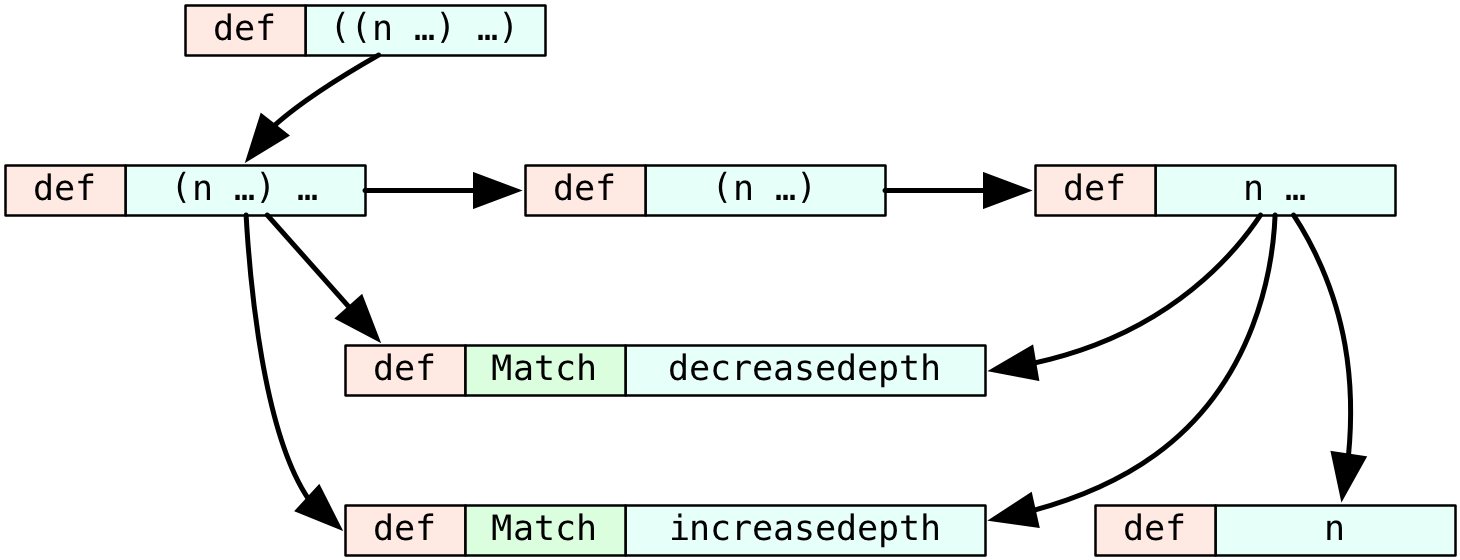
\includegraphics[scale=0.25]{ellipsis-example-callgraph.png}
\caption{Callgraph for function matching pattern \texttt{((n ...) ...)}}
\label{ellipsis-example-callgraph}
\end{figure}

Callgraph for function matching pattern \texttt{((n ...) ...)} can be seen in Figure \ref{ellipsis-example-callgraph}. Code generation algorithm generates five matching functions for this pattern:

\begin{enumerate}
\item function for pattern \texttt{((n ...) ...)}
\item function for pattern \texttt{(n ...) ...}
\item function for pattern \texttt{(n ...) }
\item function for pattern \texttt{n ... }
\item function for pattern \texttt{n}
\end{enumerate}


Figure \ref{ellipsis-example-fig-a} show state of \texttt{Match} object before beggining to match a term (red nodes) against a pattern (blue nodes). Outlined pattern nodes represent current sub-pattern being matched; and since matching hasn't begun yet the entire pattern is outlined.Same applies to the term. Initially, \texttt{Binding} instance assigned to pattern variable \texttt{n} in \texttt{Match} instance has an empty stack.

Figure \ref{ellipsis-example-fig-b} shows state of \texttt{Match} object after entering generated function for \textit{outer} ellipsis and calling \texttt{increasedepth("n")} method. This pushes empty \texttt{TermSequence} onto the stack.


Figure \ref{ellipsis-example-fig-c} shows state of \texttt{Match} object after entering generated function for \textit{inner} ellipsis and calling \texttt{increasedepth("n")} method. This pushes empty \texttt{TermSequence} onto the stack. The term now contains two \texttt{TermSequence} instances.

Figure \ref{ellipsis-example-fig-d} shows matching of term \texttt{Integer(1)}. Need to call \texttt{addtobinding} method with \texttt{"n"} and \texttt{Integer(1)} as arguments. Since topmost term on the stack is \texttt{TermSequence}, \texttt{Integer(1)} is appended to it.

Figures \ref{ellipsis-example-fig-e} and \ref{ellipsis-example-fig-f} call \texttt{addtobinding} with \texttt{Float(2.01)} and \texttt{Integer(3)}. Both terms are appended to the topmost \texttt{TermSequence} on the stack.

All terms in \texttt{TermSequence} have been consumed. Figure \ref{ellipsis-example-fig-g} shows state of the match object after calling \texttt{decreasedepth("n")}. Since the stack contains to \texttt{TermSequence} instances, topmost one is removed from stack and appended to the first \texttt{TermSequence}. Function for \textit{inner} ellipsis is exited.

Now, remaining empty term sequence has to be matched, as seen in Figure \ref{ellipsis-example-fig-h}.

Figure \ref{ellipsis-example-fig-i} shows state of \texttt{Match} object after entering generated function for \textit{inner} ellipsis. Empty \texttt{TermSequence} instance is pushed onto the stack.

However, since term sequence is empty, function for \texttt{Number} pattern cannot be called. Figure \ref{ellipsis-example-fig-j} shows state of the \texttt{Match} object after calling \texttt{decreasedepth("n")}. Since stack contains two \texttt{TermSequence} instances, topmost one is popped from the stack and appended to previous \texttt{TermSequence}. Function for \textit{inner} ellipsis is exited.

Finally, there's no more terms to match in outermost sequence and \texttt{decreasedepth("n")} has to be called, as shown in Figure \ref{ellipsis-example-fig-k}. Since the stack only contains a single term, \texttt{decreasedepth} has no effect.

Assignment \texttt{n = ((1 2 3)())} is matched, as expected.

One may notice that this example doesn't cover non-determinism when matching patterns under ellipsis. When matching term \texttt{(1 2 3)} against pattern \texttt{n ...} (as shown in Figures \ref{ellipsis-example-fig-d}, \ref{ellipsis-example-fig-e}, \ref{ellipsis-example-fig-f}), the matches shown in Figure \ref{ellipsis-example-matches-1} are returned. Recall that when calling a function that matches \texttt{TermSequence}, \texttt{head} and \texttt{tail} are set to zero and the length of \texttt{TermSequence}, in this case three. Function for \texttt{n ...} is then called, \texttt{increasedepth} method is called on \texttt{match} instance and it is placed into the queue. Match is then popped from the queue, add function for pattern \texttt{n} is called with complete copy of the match. Such repeated copying and calling \texttt{decreasedepth} for each resulting match produces matches shown in Figure \ref{ellipsis-example-matches-1}. Now, when exiting function for pattern \texttt{(n ...)}, only accept matches where \texttt{head=tail}, and there's only such match.

When control flow returns to function for pattern \texttt{(n ...) ...)}, the only returned match is added to the queue. Queue at this point contains a single match. This match is dequeued, and function for pattern \texttt{(n ...) is called} with term \texttt{()}. \texttt{head} and \text{tail} are set to zero and function for pattern \texttt{n ...} is called. \texttt{increasedepth} is called. Since term \texttt{()} contains no numbers, the only possible match returned by this function is shown in Figure \ref{ellipsis-example-matches-2}.

Finally, \textit{outer} ellipsis produces matches shown in Figure \ref{ellipsis-example-matches-3} When returning from function for pattern \texttt{((n ...) ...)}, two of the matches are discarded because \texttt{head != tail}.


\begin{figure}[H]
\caption{Lifetime of match object}
%\begin{adjustwidth}{-1cm}{1cm}
\fbox{
	\begin{subfigure}{0.5\linewidth}
		\raisebox{5mm}{
			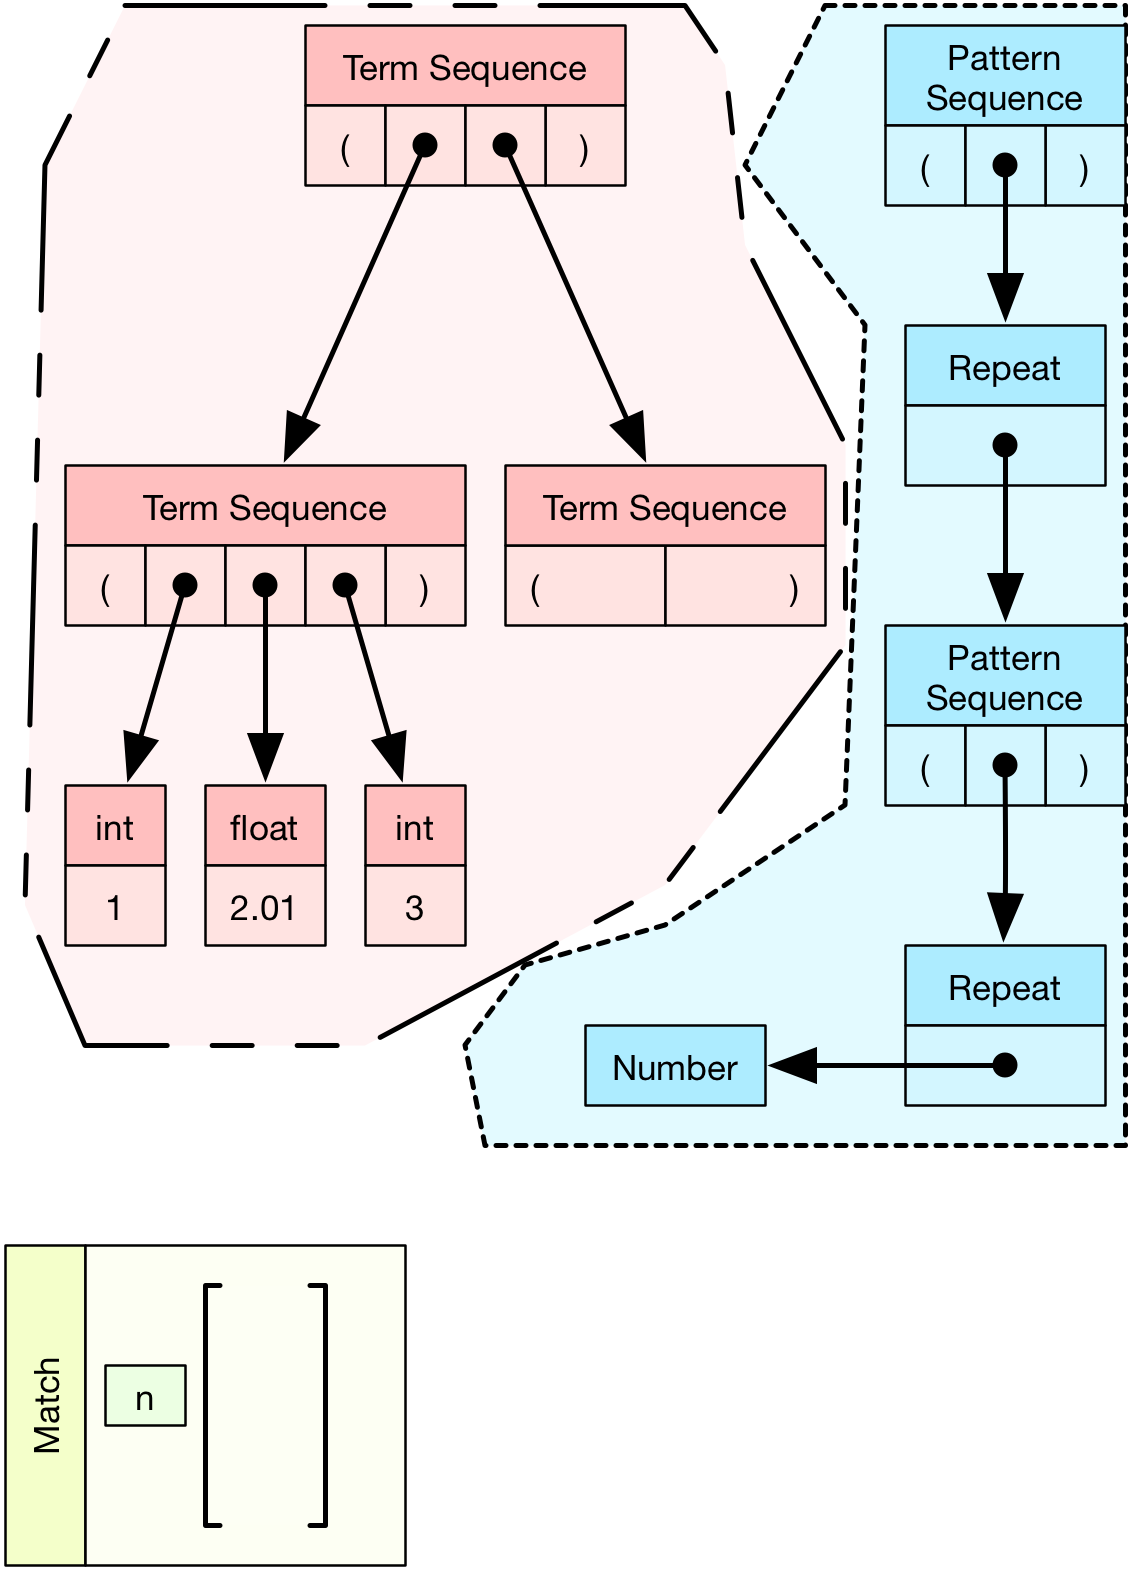
\includegraphics[scale=0.152]{ellipsis-example-fig-a.png}
		}
		\caption{Before matching the pattern.}
		\label{ellipsis-example-fig-a}
	\end{subfigure}
	\begin{subfigure}{0.5\linewidth}
		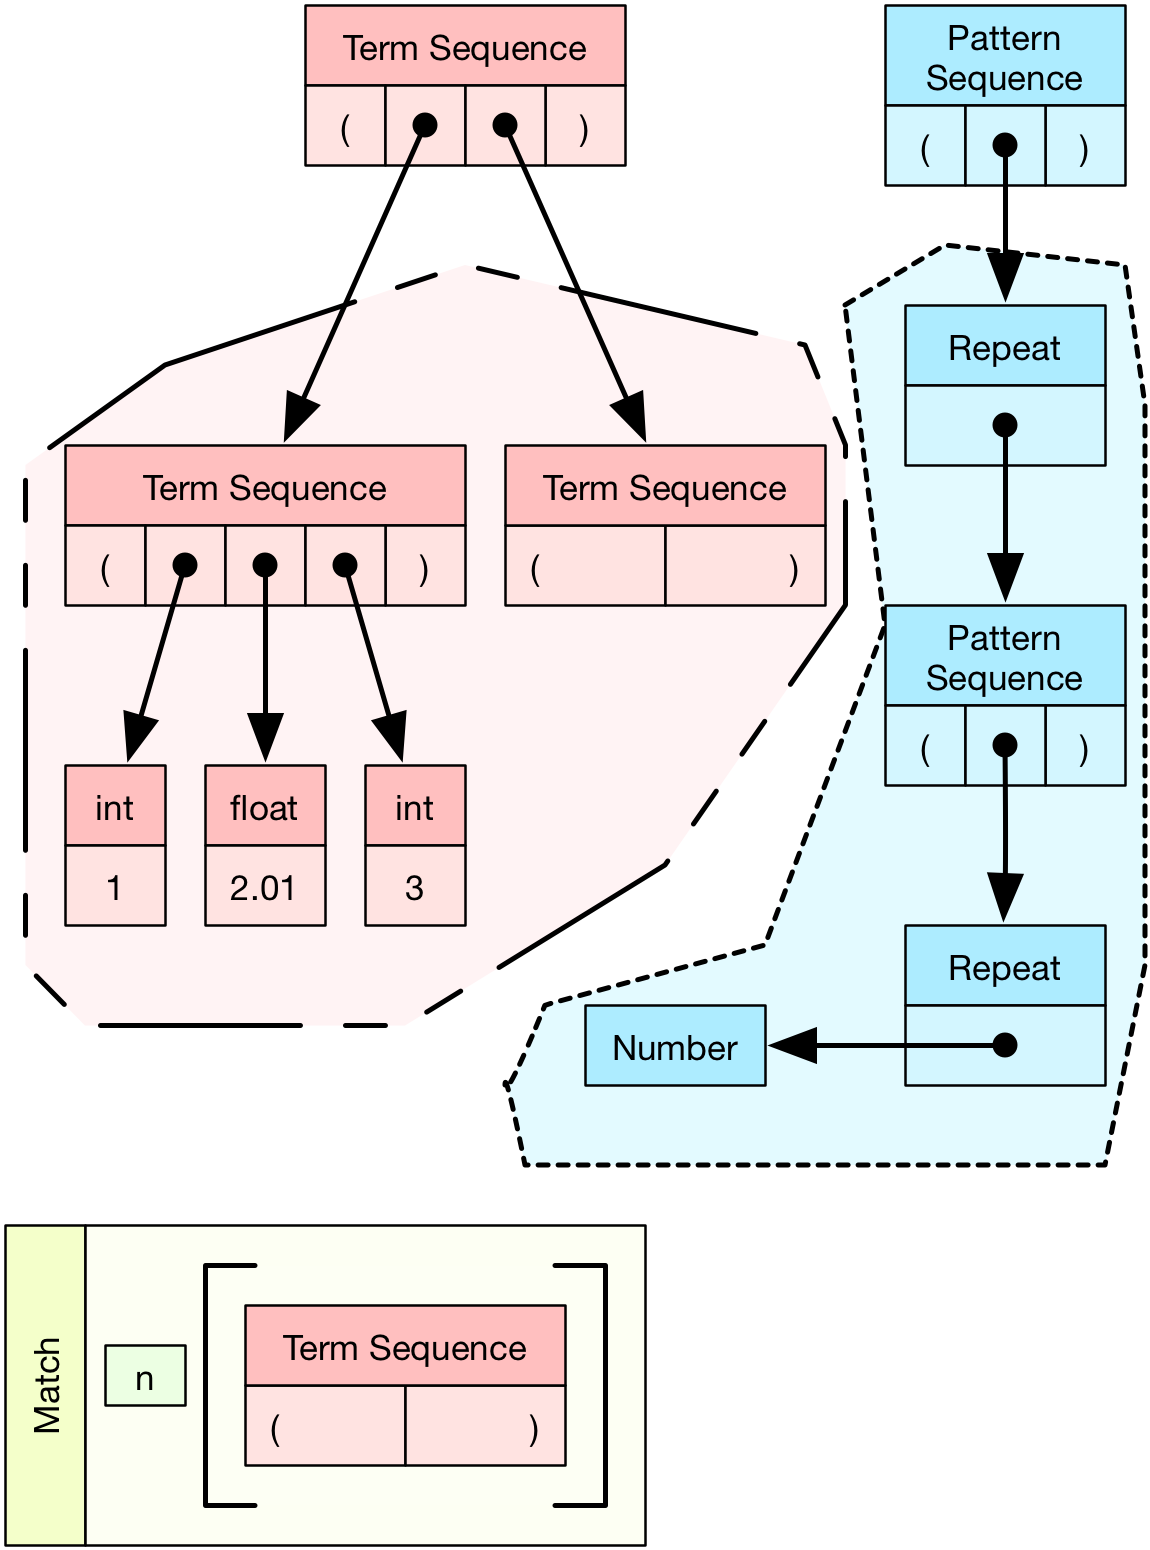
\includegraphics[scale=0.152]{ellipsis-example-fig-b.png}
		\caption{Enter outer ellipsis and \texttt{increasedepth("n")}.}
		\label{ellipsis-example-fig-b}
	\end{subfigure}
}

\fbox{
	\begin{subfigure}{0.5\linewidth}
		\raisebox{19mm}{
			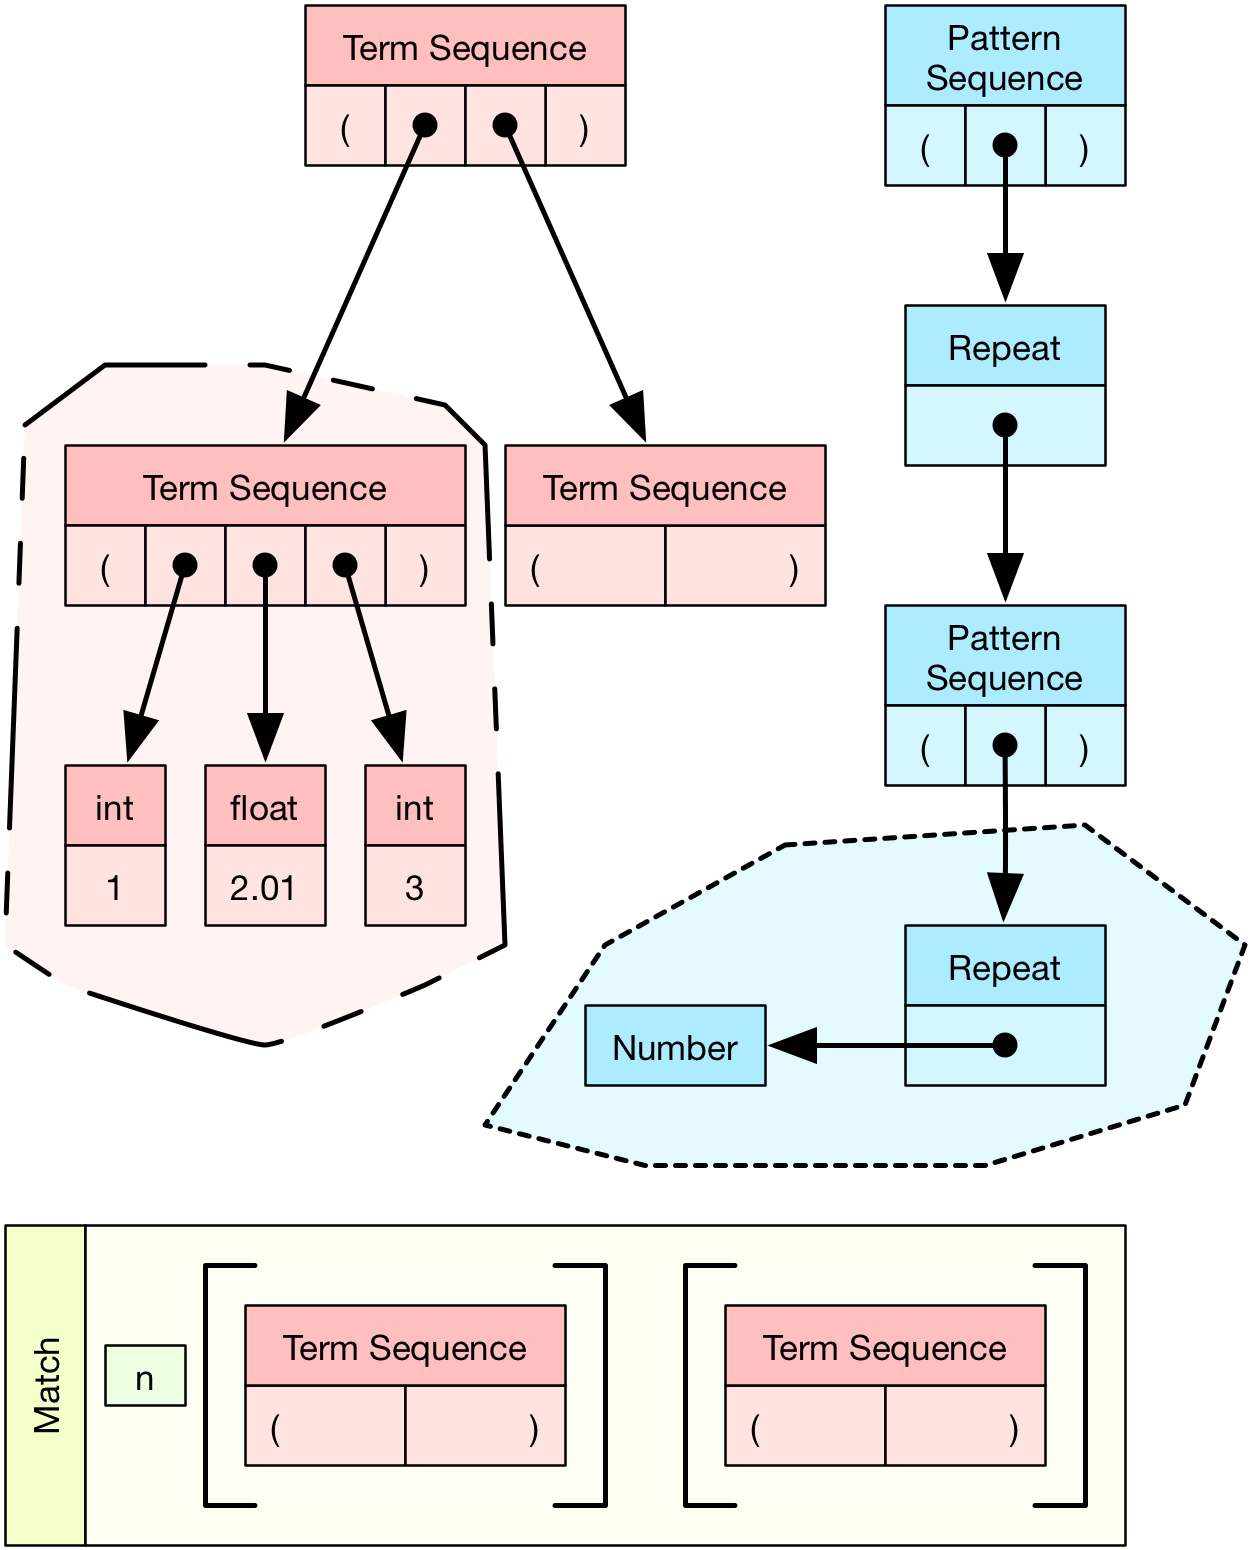
\includegraphics[scale=0.152]{ellipsis-example-fig-c.png}
		}
		\caption{Enter inner ellipsis and \texttt{increasedepth("n")}.}
		\label{ellipsis-example-fig-c}
	\end{subfigure}
	\begin{subfigure}{0.5\linewidth}
		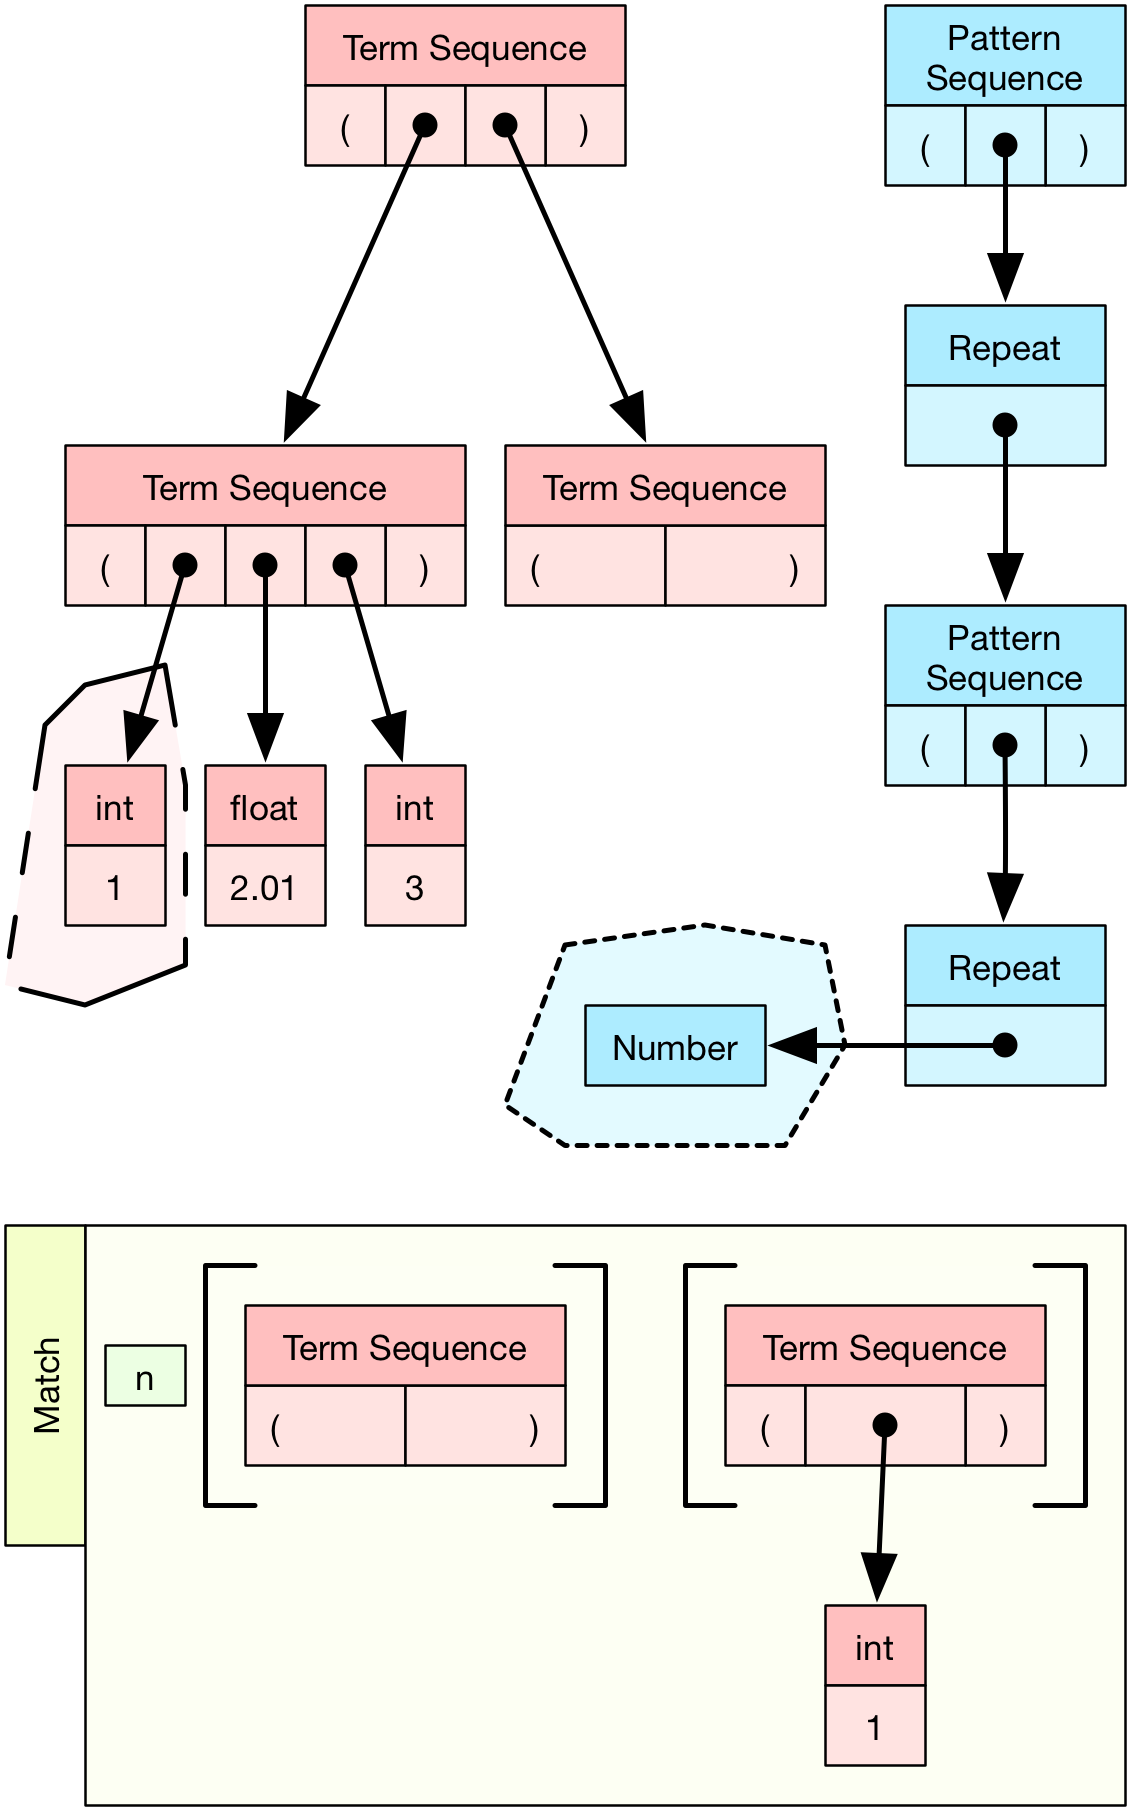
\includegraphics[scale=0.152]{ellipsis-example-fig-d.png}
		\caption{\texttt{addtobinding("n", Integer(1))}}
		\label{ellipsis-example-fig-d}
	\end{subfigure}
}

%\end{adjustwidth}
\end{figure}

\begin{figure}[H]\ContinuedFloat
\fbox{
	\begin{subfigure}{0.5\linewidth}
		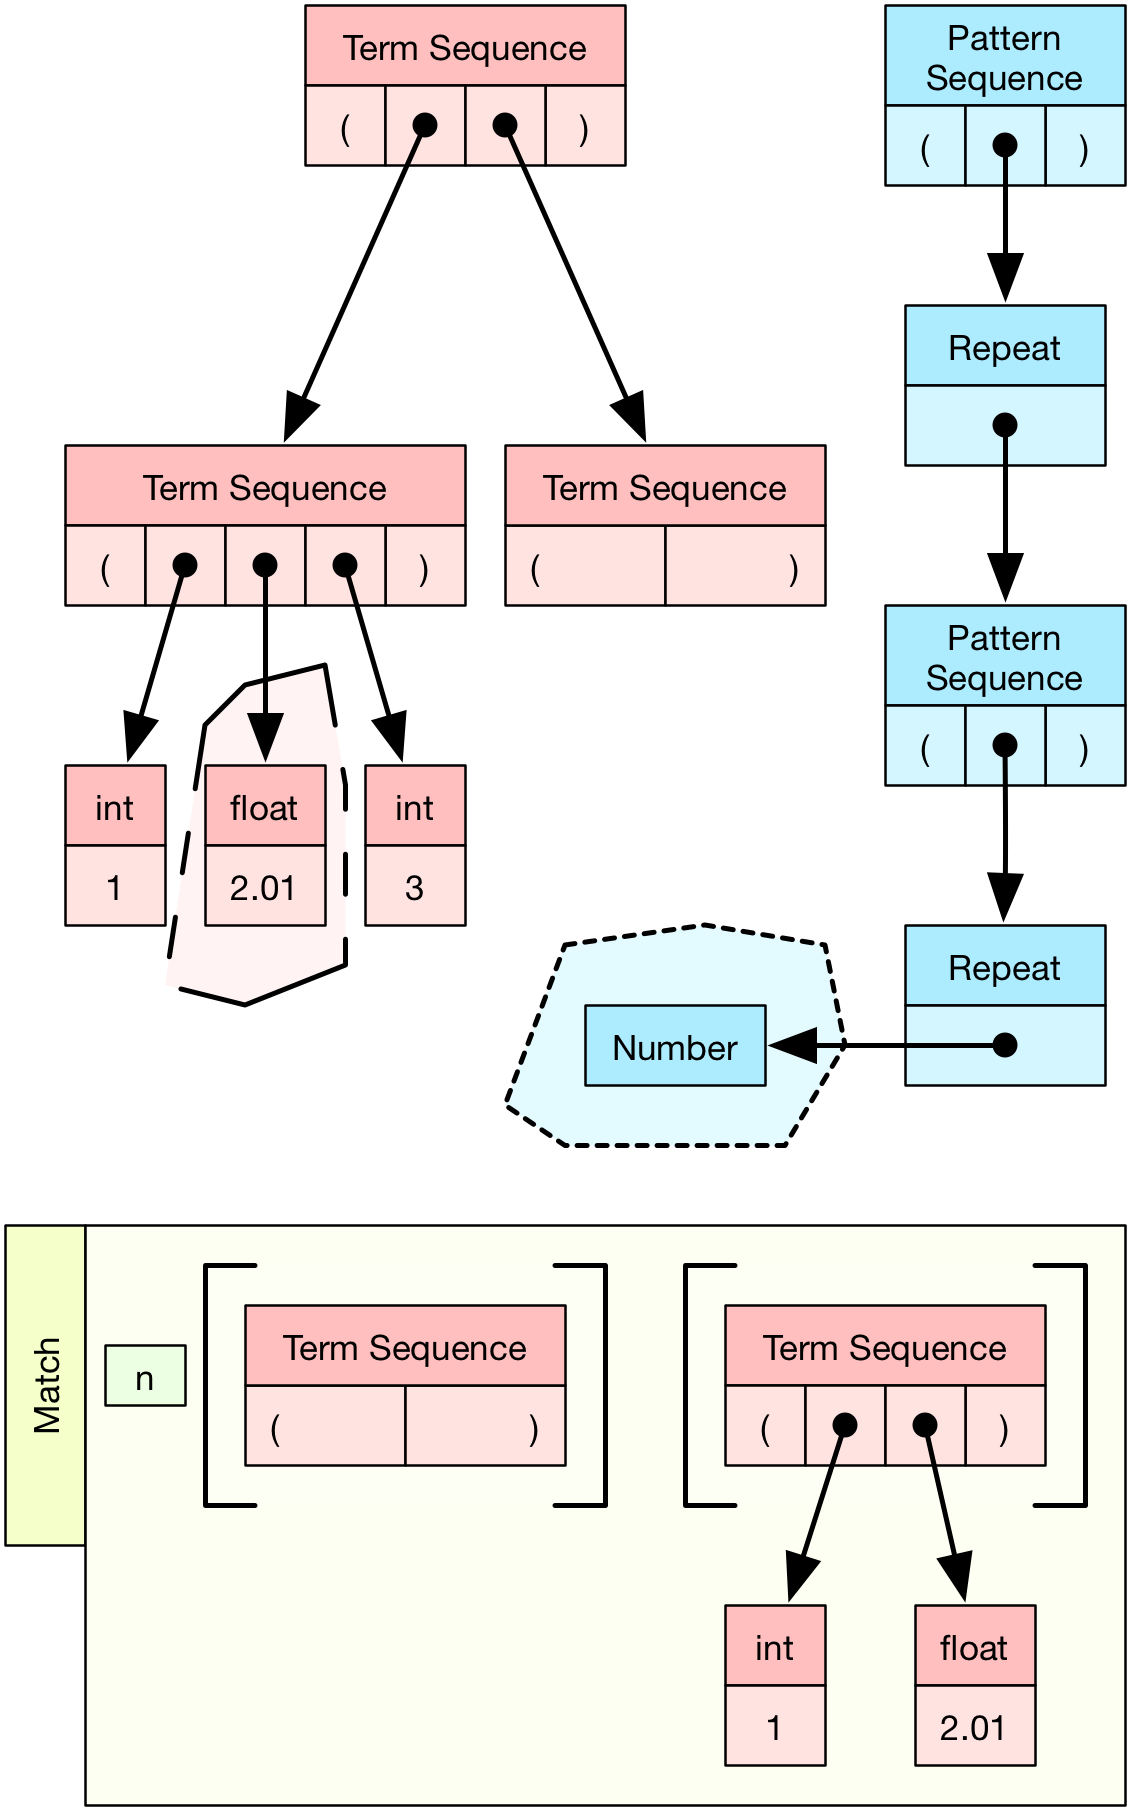
\includegraphics[scale=0.152]{ellipsis-example-fig-e.png}
		\caption{\texttt{addtobinding("n", Float(2.01))}}
		\label{ellipsis-example-fig-e}
	\end{subfigure}
	\begin{subfigure}{0.5\linewidth}
		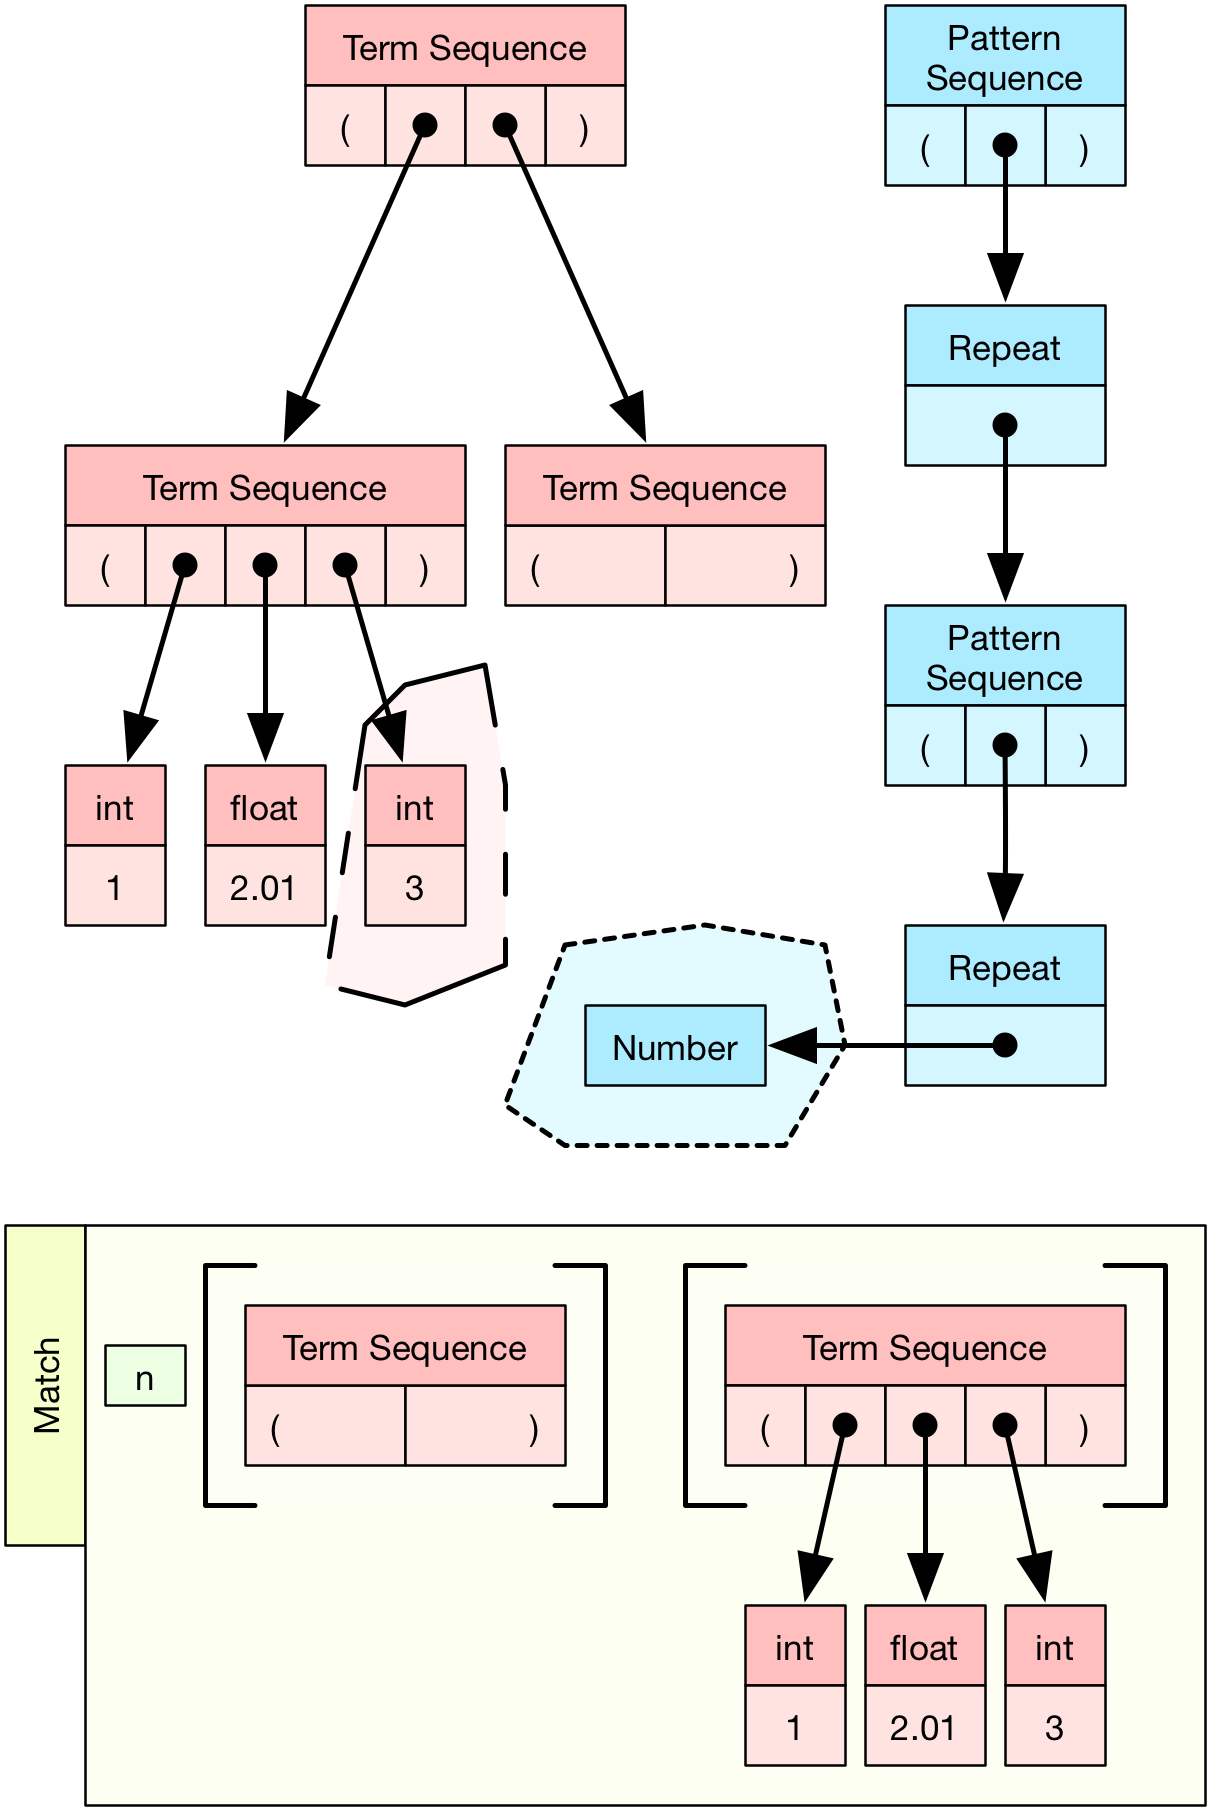
\includegraphics[scale=0.152]{ellipsis-example-fig-f.png}
		\caption{\texttt{addtobinding("n", Integer(3))}}
		\label{ellipsis-example-fig-f}
	\end{subfigure}
}
\fbox{
\begin{subfigure}{0.5\linewidth}
	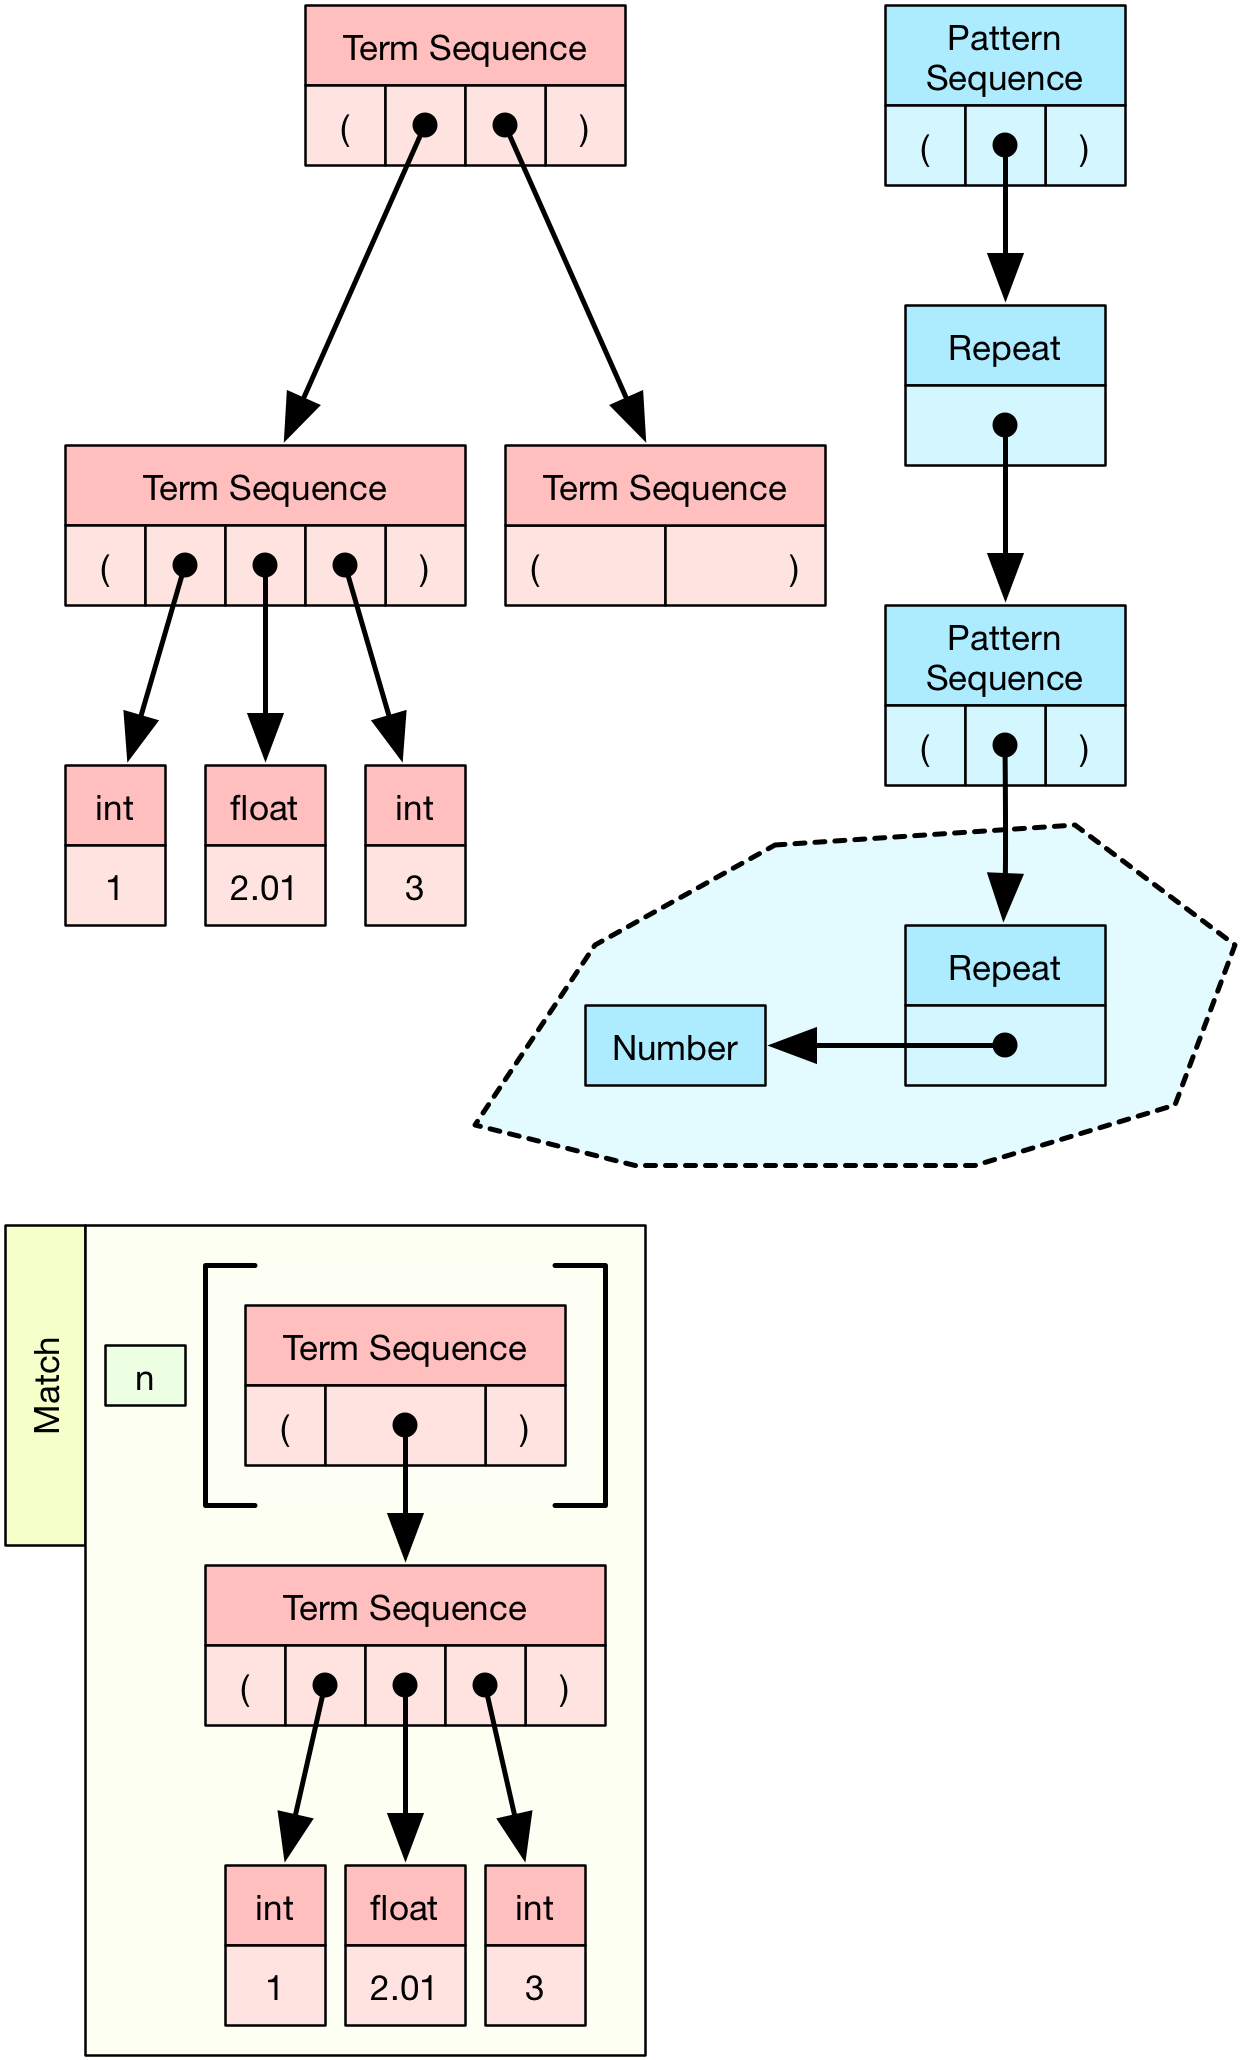
\includegraphics[scale=0.152]{ellipsis-example-fig-g.png}
	\caption{\texttt{decreasedepth("n")} and leave inner ellipsis.}
	\label{ellipsis-example-fig-g}
\end{subfigure}
\begin{subfigure}{0.5\linewidth}
	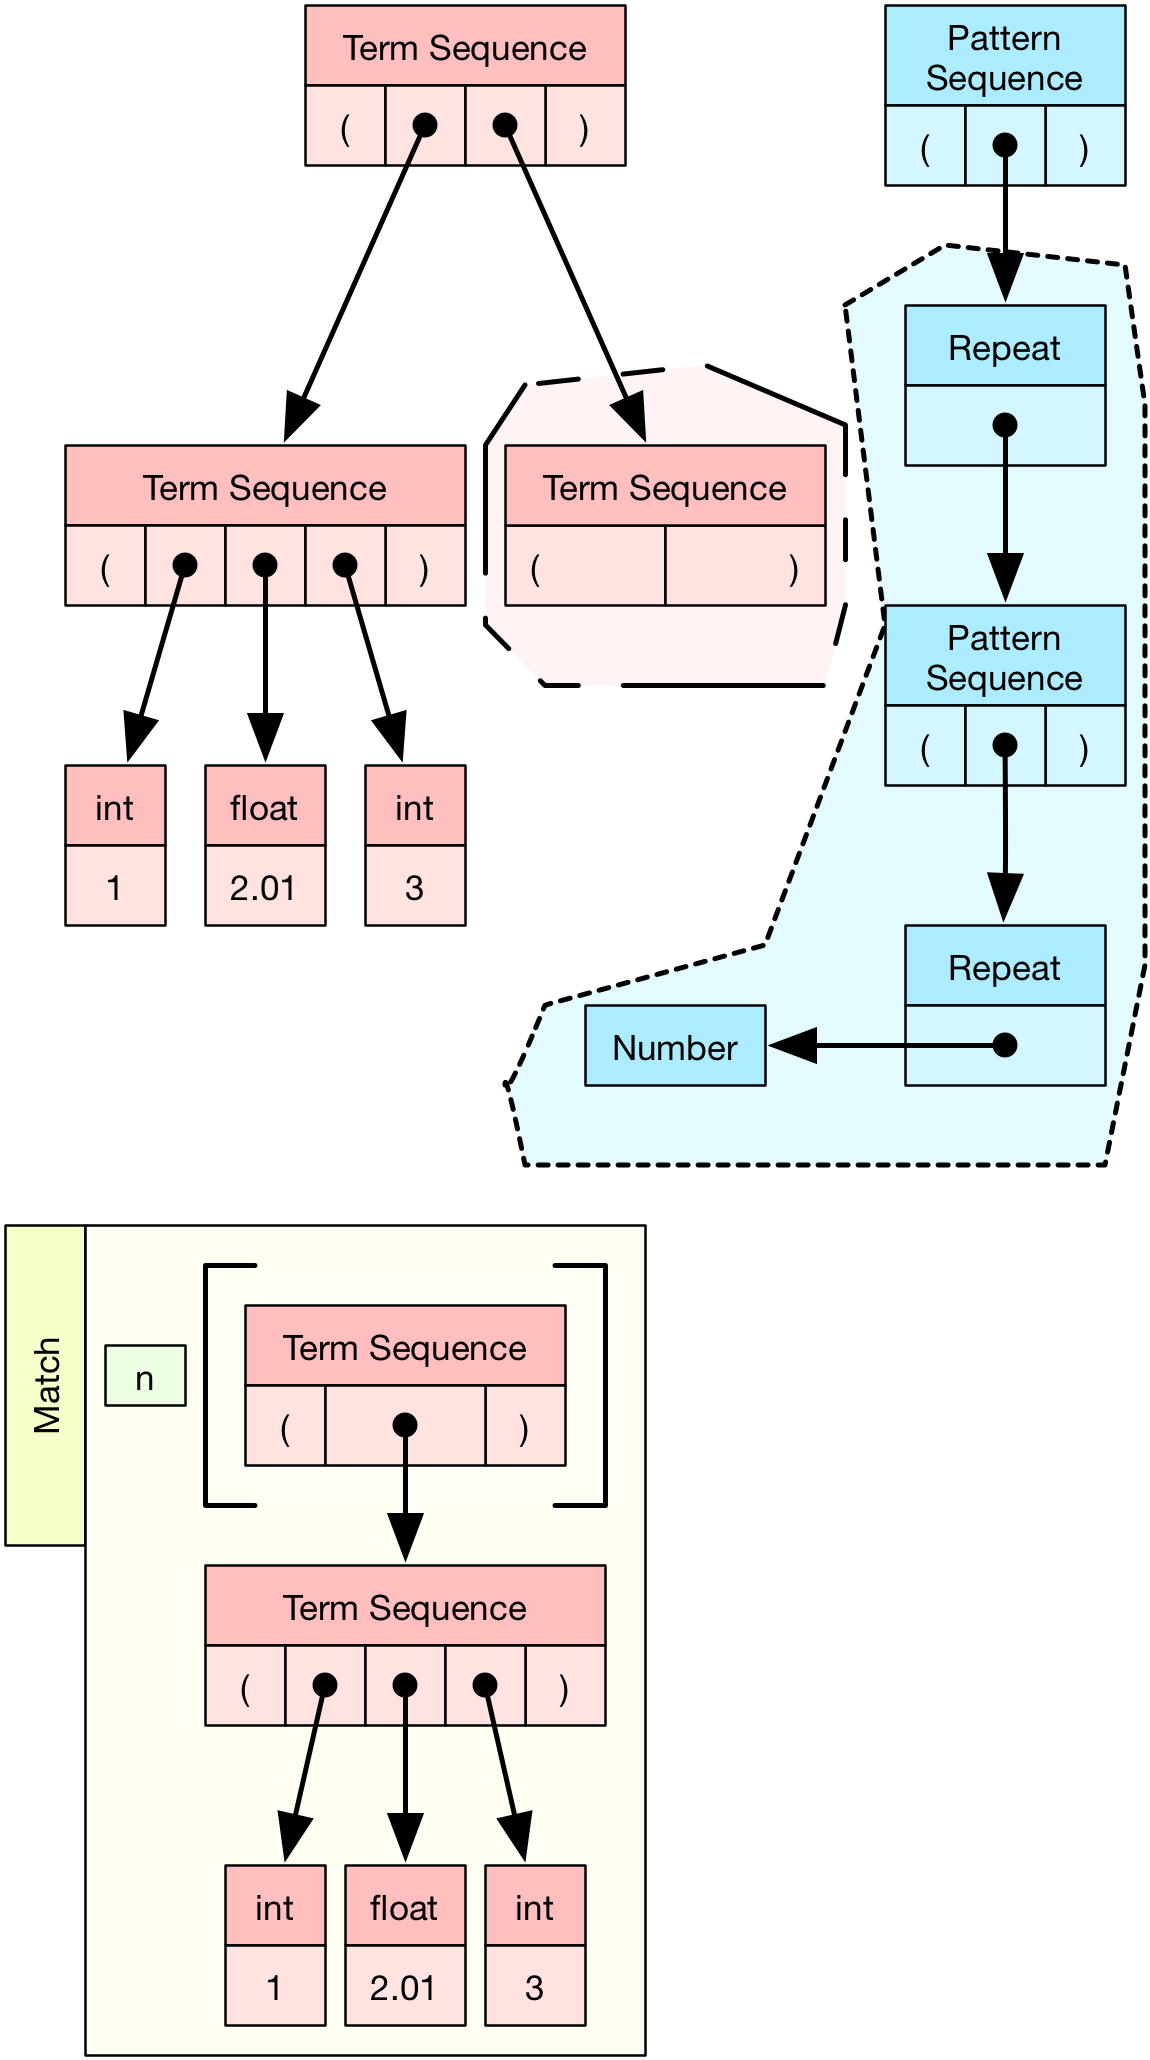
\includegraphics[scale=0.152]{ellipsis-example-fig-h.png}
	\caption{Start processing the next term in the sequence.}
	\label{ellipsis-example-fig-h}
\end{subfigure}
}
\end{figure}
\begin{figure}[H]\ContinuedFloat
\fbox{
	\begin{subfigure}{0.5\linewidth}
		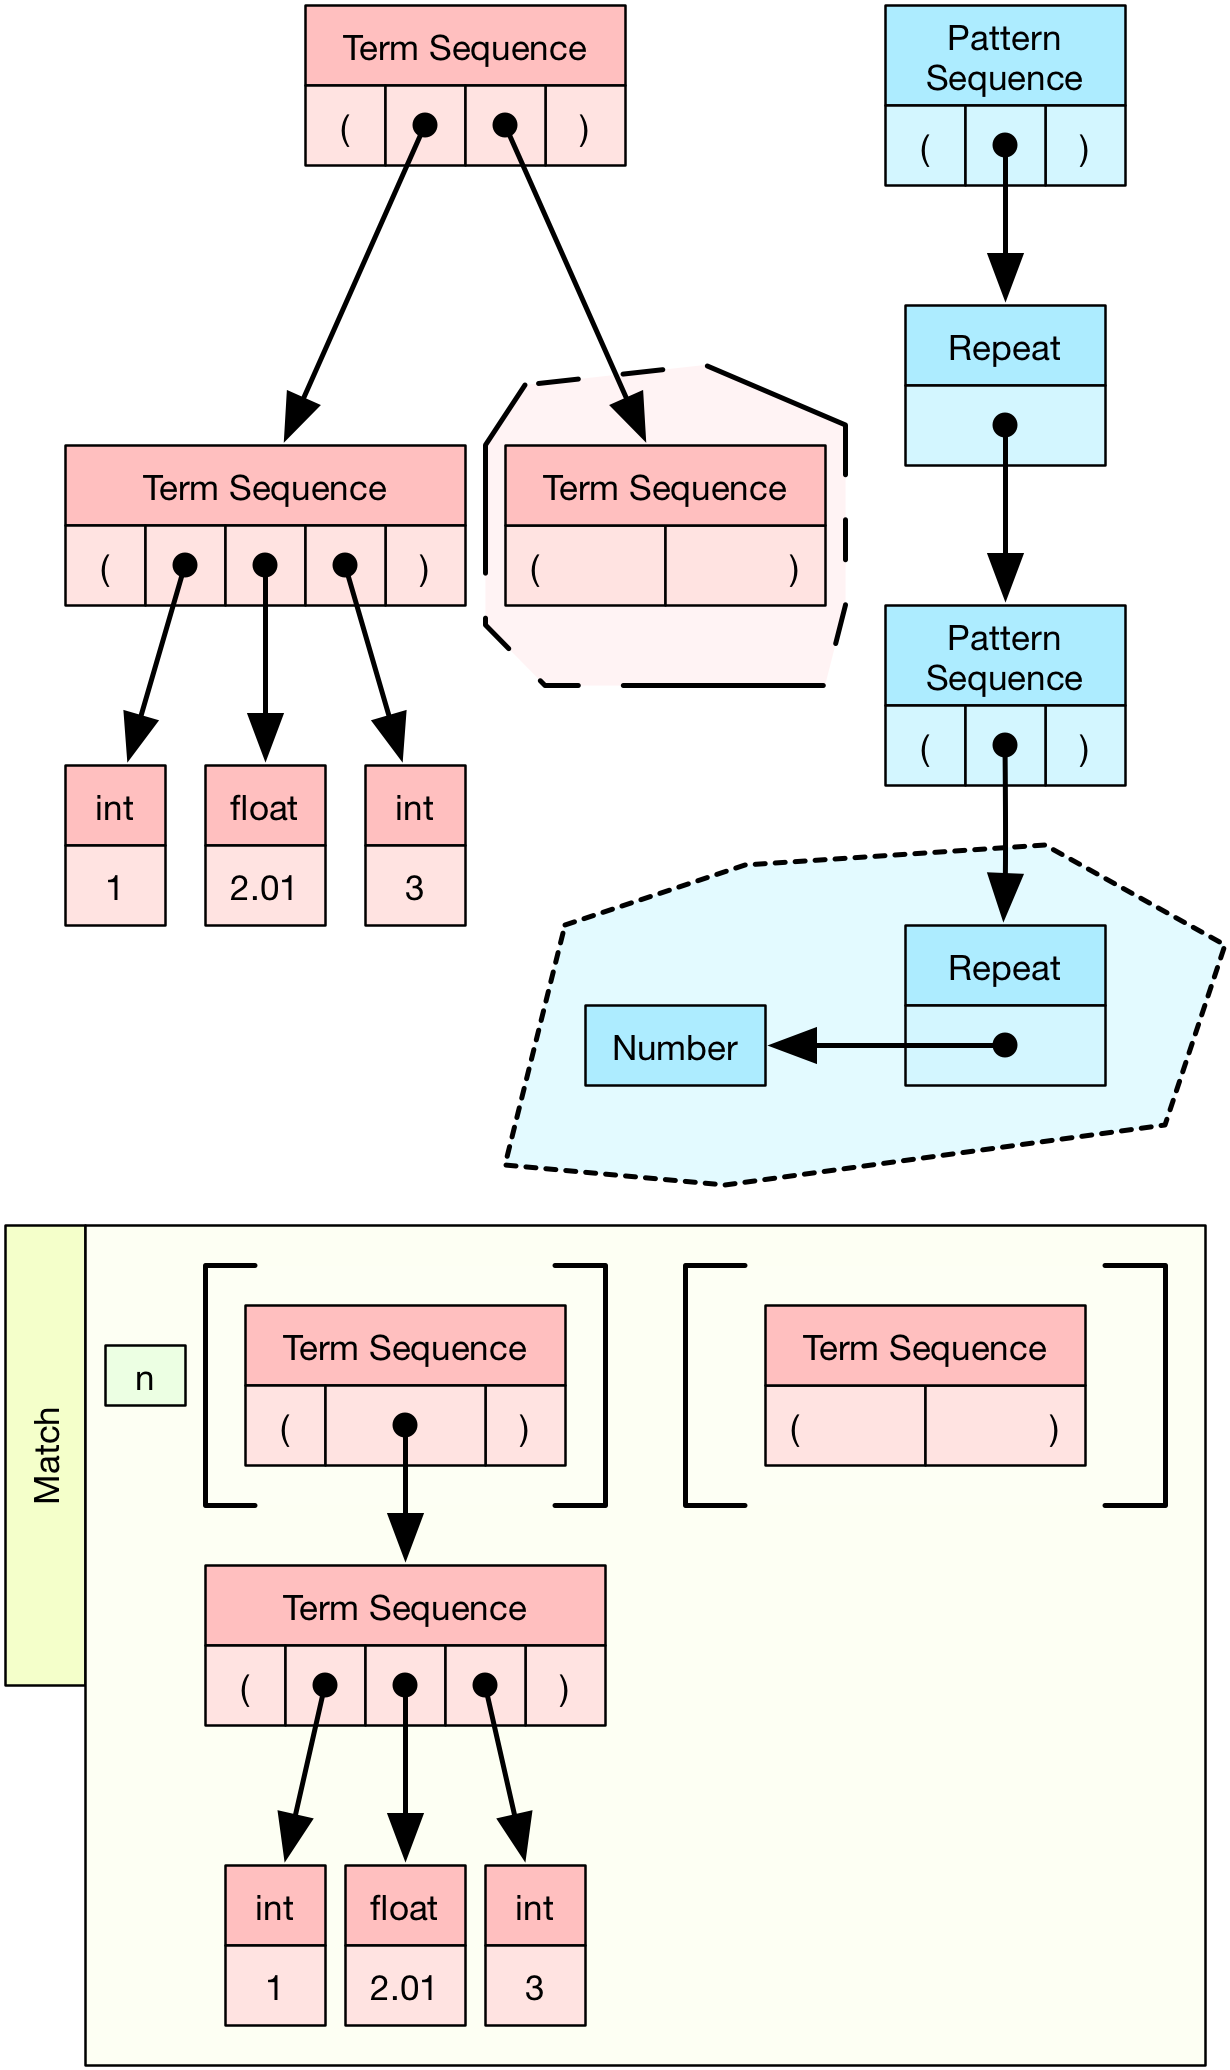
\includegraphics[scale=0.152]{ellipsis-example-fig-i.png}
		\caption{\texttt{increasedepth("n")} after entering inner ellipsis.}
		\label{ellipsis-example-fig-i}
	\end{subfigure}
	\begin{subfigure}{0.5\linewidth}
		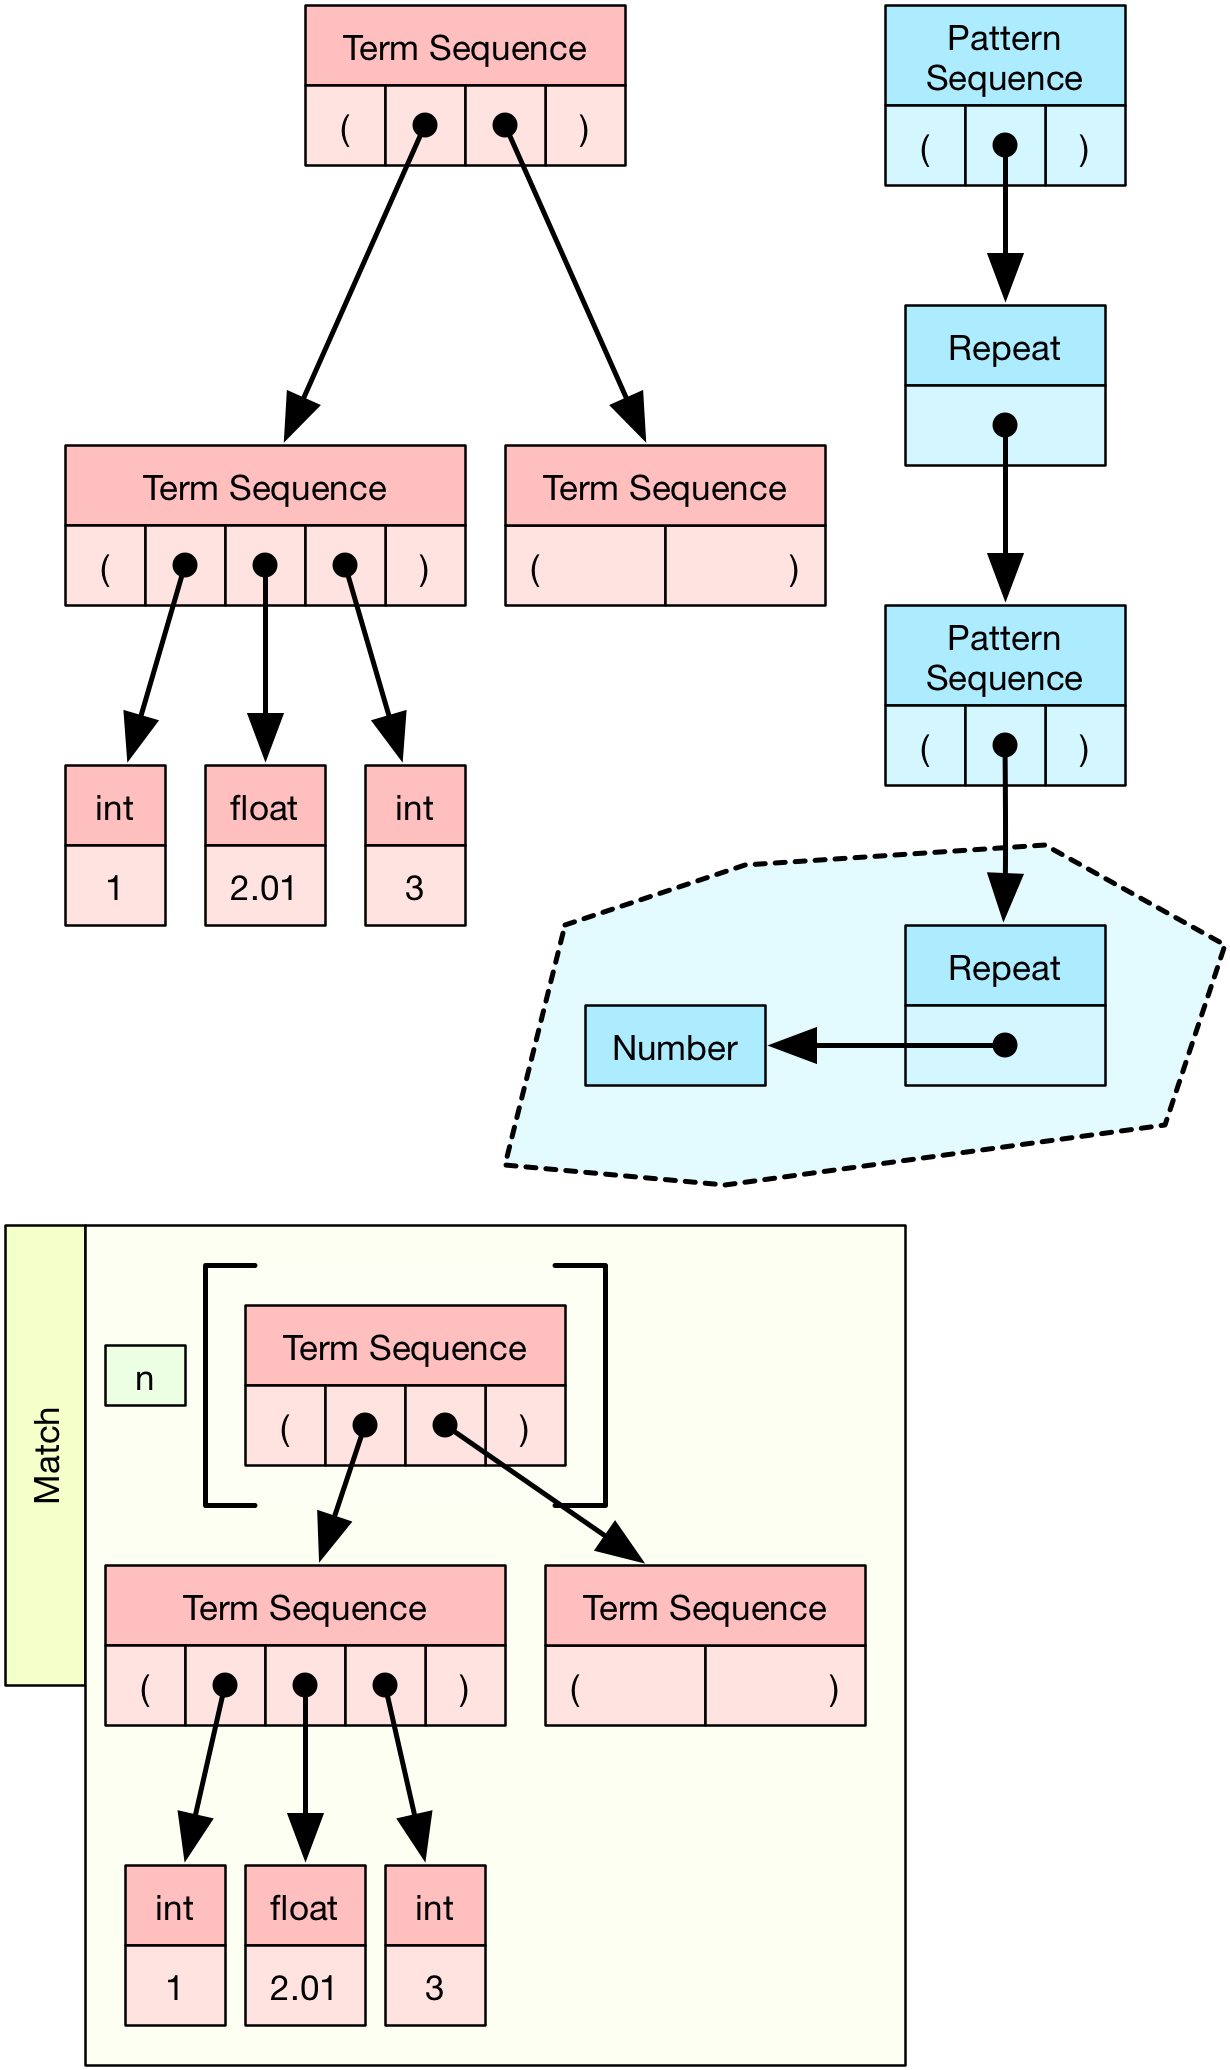
\includegraphics[scale=0.152]{ellipsis-example-fig-j.png}
		\caption{\texttt{decreasedepth("n")} and leave inner ellipsis.}
		\label{ellipsis-example-fig-j}
	\end{subfigure}
}

\fbox{
	\begin{subfigure}{0.5\linewidth}
		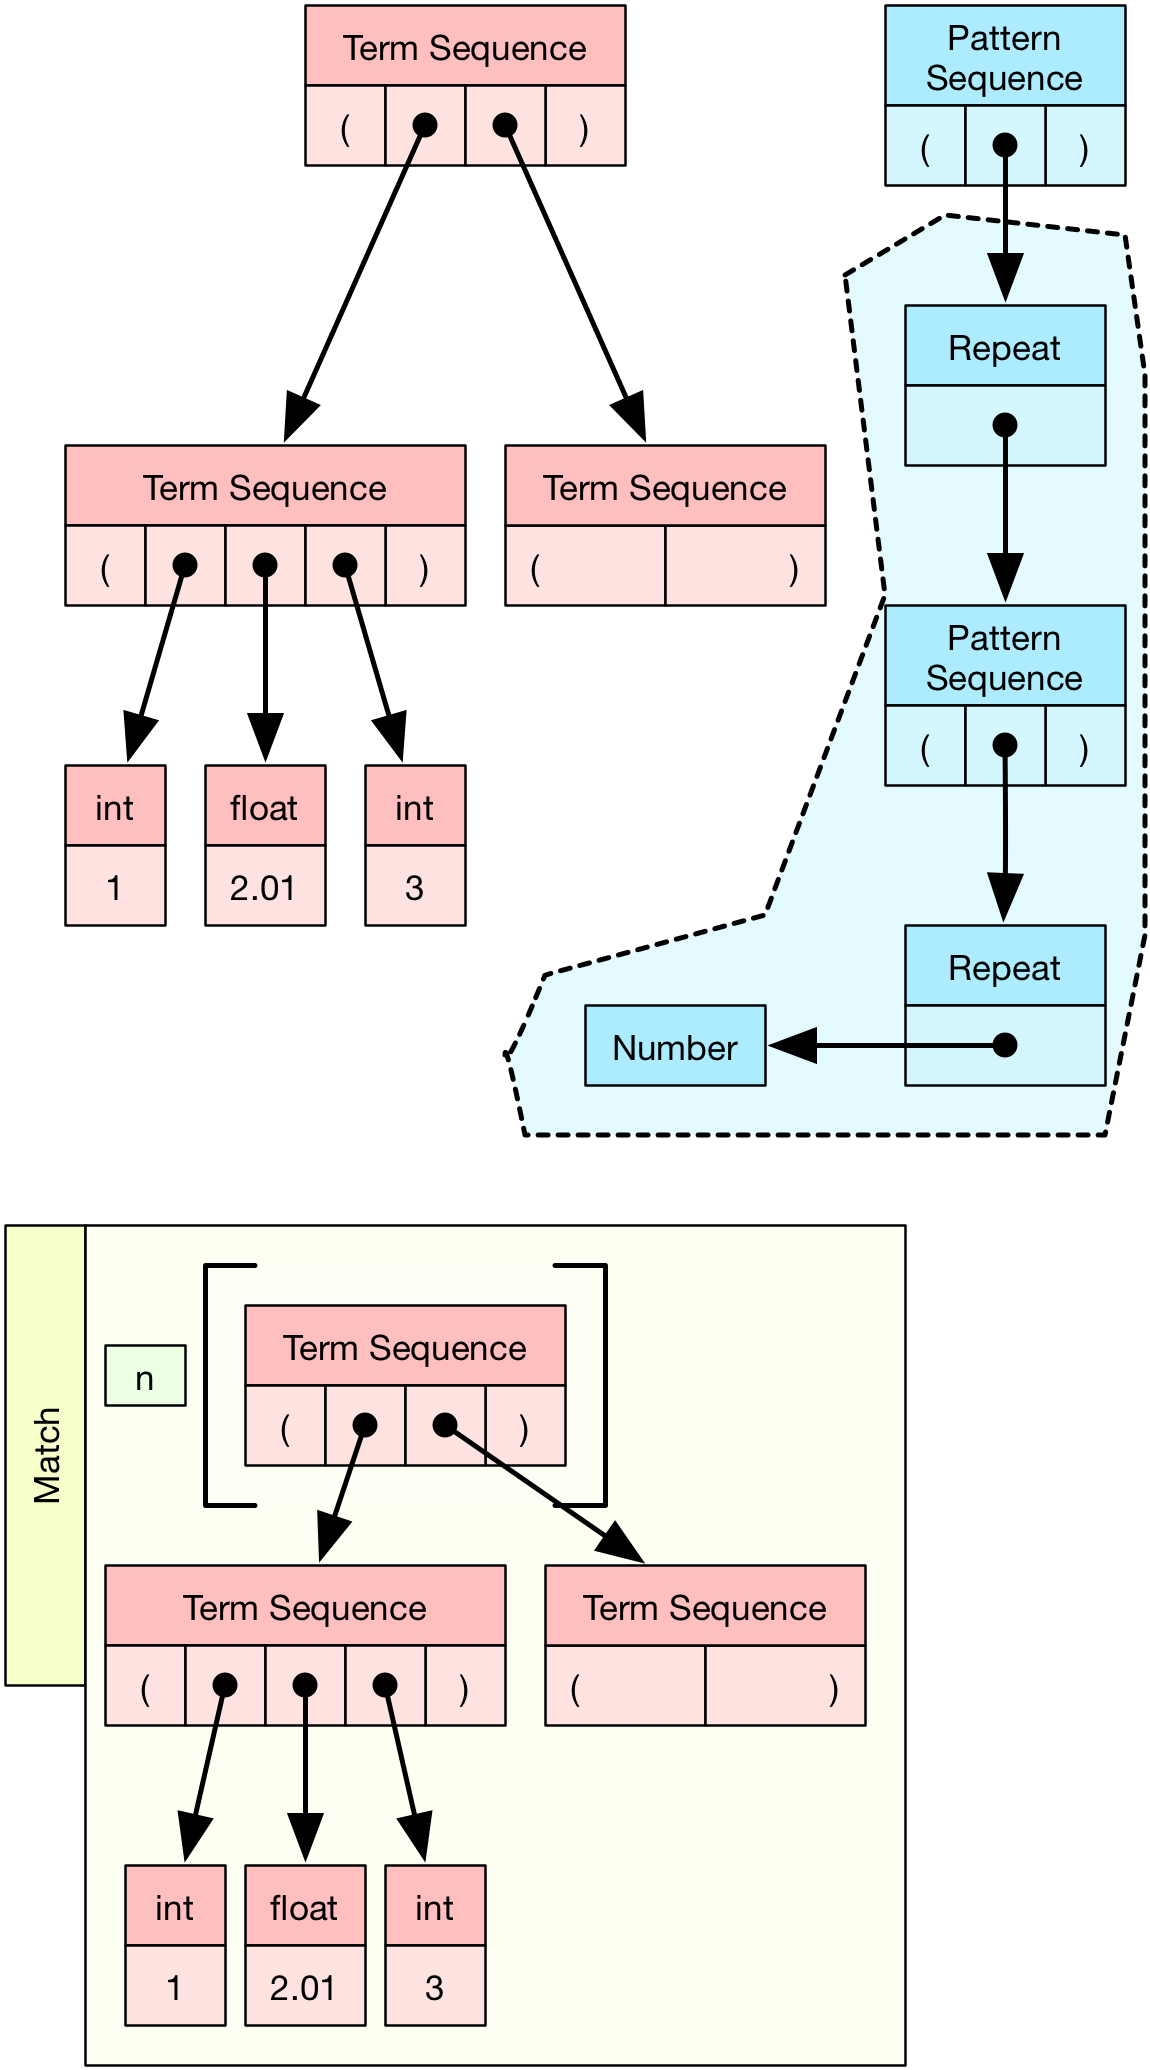
\includegraphics[scale=0.152]{ellipsis-example-fig-k.png}
		\caption{\texttt{decreasedepth("n") and leave outer ellipsis}.}
		\label{ellipsis-example-fig-k}
	\end{subfigure}
}

\end{figure}

\begin{figure}[h]
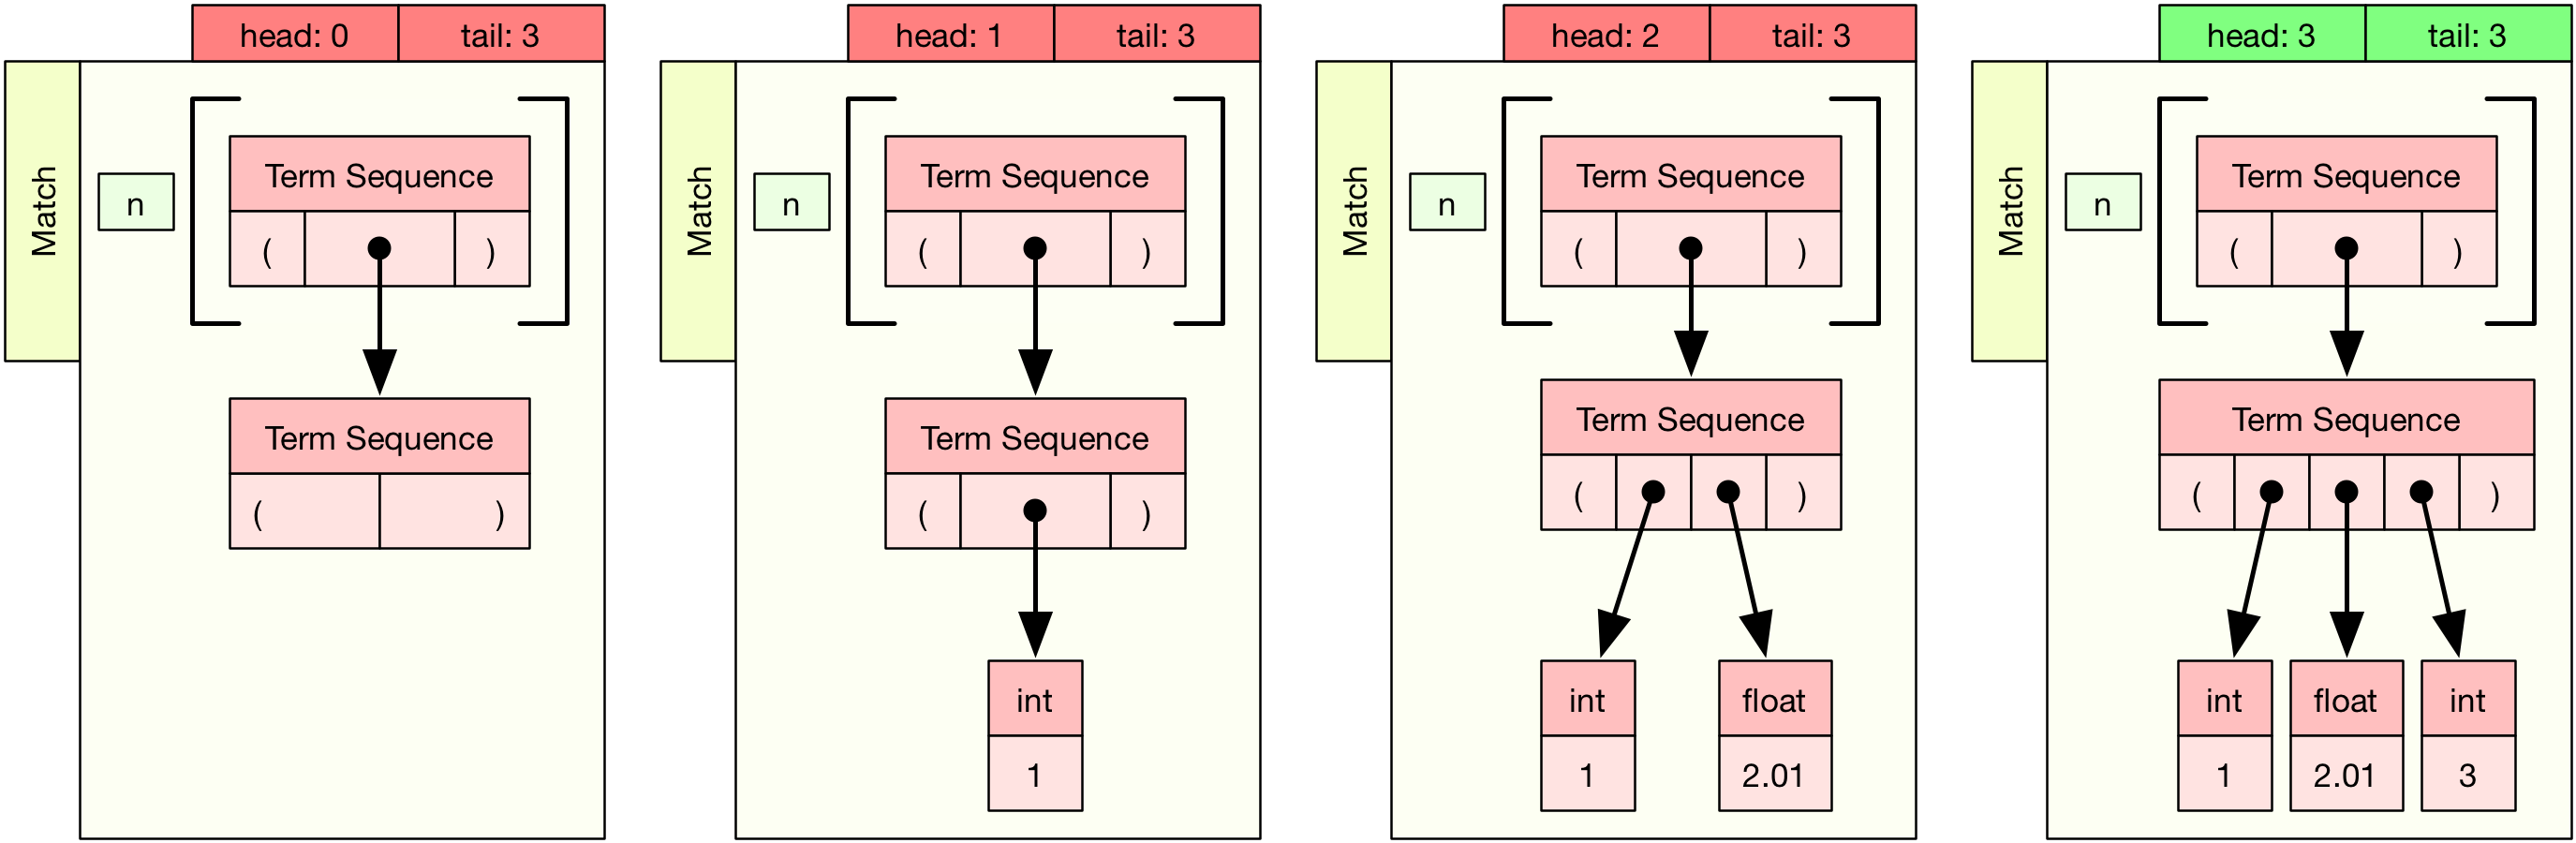
\includegraphics[scale=0.152]{ellipsis-example-matches-1.png}
\caption{Matches returned after matching term \texttt{(1 2 3)} against pattern \texttt{n ...}}
\label{ellipsis-example-matches-1}
\end{figure}


\begin{figure}[h]
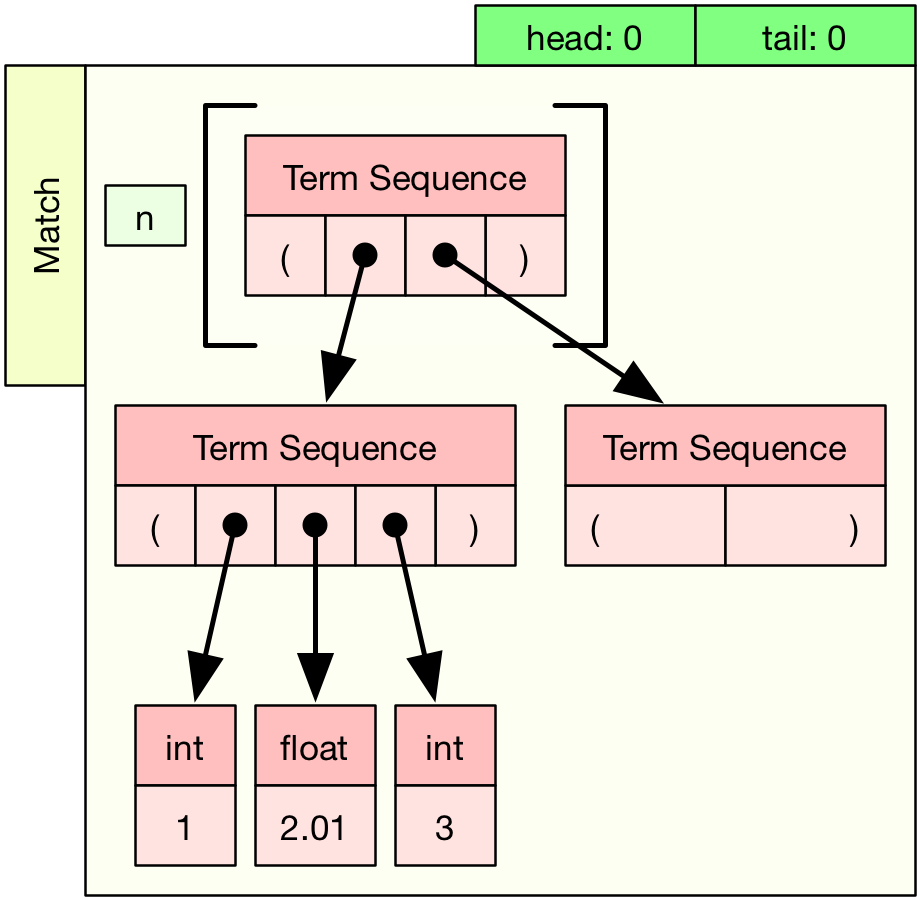
\includegraphics[scale=0.152]{ellipsis-example-matches-2.png}
\caption{Matches returned after matching term \texttt{()} against pattern \texttt{n ...}}
\label{ellipsis-example-matches-2}
\end{figure}

\begin{figure}[h]
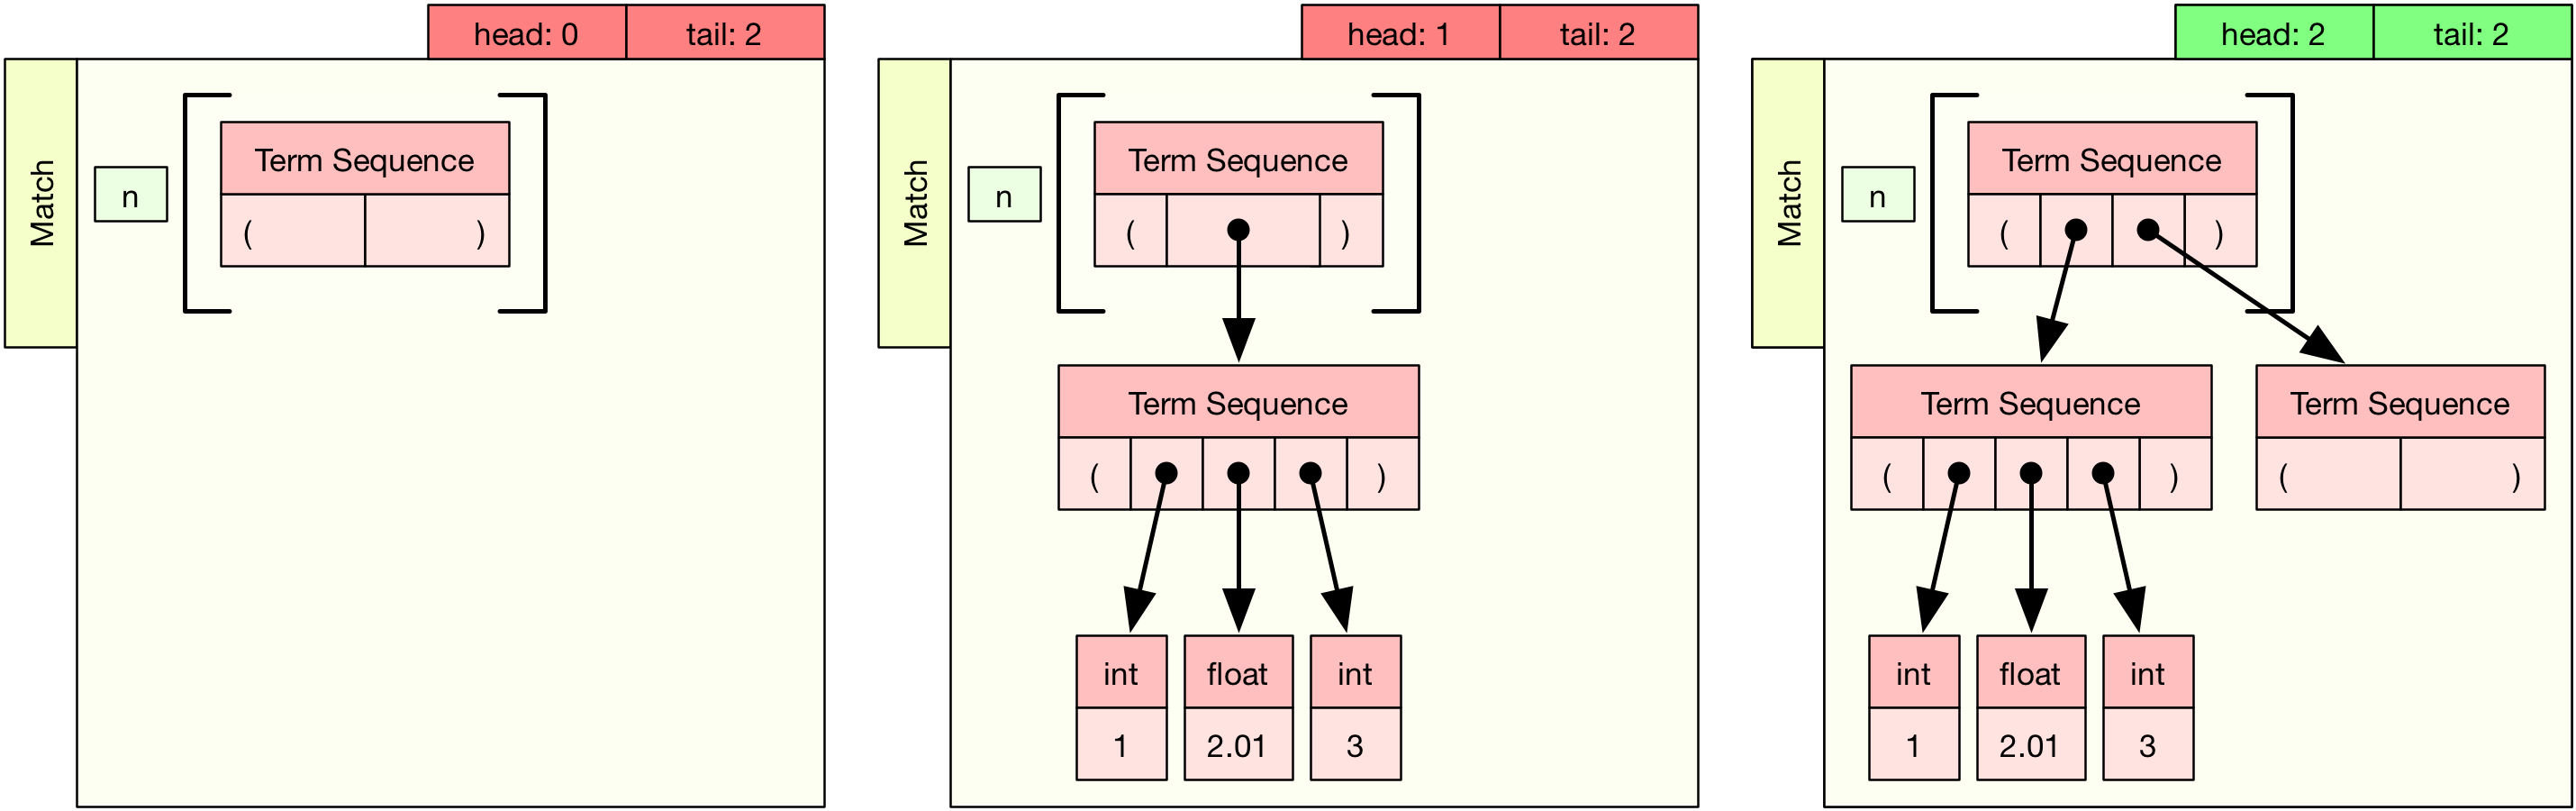
\includegraphics[scale=0.152]{ellipsis-example-matches-3.png}
\caption{Matches returned after matching term \texttt{((1 2 3)())} against pattern \texttt{(n ...) ...} }
\label{ellipsis-example-matches-3}
\end{figure}



\subsection{Match Function: InHole pattern}
In-hole pattern consists of two patterns. The term is traversed recursively trying to find a subterm that matches the second pattern. If such subterm is found, the term is copied from previously mentioned subterm all the way to the root and subterm is replaced with term `hole`. Copying is needed because original term must be left intact.

For recursive term traversal a path from root of the term to possible subterm matching the second pattern is maintained. This allows for only copying terms/subterms that will be affected by `hole` substitution instead of copying the entire term.

Due to possible non-determinism, `match` object must remain unmodified. For both patterns of `in-hole`, separate `Match` objects are created and initialized with appropriate meta-variables. Upon successful matching by both procedures, Cartesian product between matches of both lists is computed and results are inserted into a copy of initial `match` object. By construction, all meta-variables of `Match` objects are unique.


\subsection{Top-Level Matching Function}

This procedure creates `Match` object, initializes it with assignable symbols seen in the actual pattern and calls appropriate matching procedure. `head` and `tail` parameters are set to zero and one, respectively. Since matching procedure returns a list of `(match, head ,tail)` tuples, `Match` objects are filtered out and returned.

